% \chapter{基于内存压力的自动卸载框架}
% \label{chap:基于内存压力的自动卸载框架}
% 在\ref{chap:基于同步内存回收的内存压力量化算法的设计与实现}中,已将同步内存回收量化为内存压力。基于量化的压力值,用户态的内存压力感知卸载框架可以主动将冷页面卸载到异构后端。本章将介绍基于proc文件系统的mpfs实现、基于内存压力的工作集估计算法以及基于访问距离的匿名页和文件页的平衡算法的设计与实现。


% % \section{内存压力文件系统的实现}
% % \label{sec:mpfs_implementation}

% % 基于\ref{sec:基于同步回收延迟的内存压力量化实现}章节实现的内存压力量化模型,可以实时的计算工作集,计算工作集需要不同的策略。本节构建用户态调控接口以实现冷页面的动态卸载机制。选择用户态实现方案可有效提升策略迭代效率,同时支持基于 QoS 需求的差异化策略配置。

% % \subsection{proc 文件系统架构分析}

% % proc 文件系统作为内核与用户态间的标准交互接口,其设计具有以下核心特征:

% % \begin{itemize}
% %     \item \textbf{动态生成机制:} 文件节点根据内核运行时状态实时构建
% %     \item \textbf{虚拟存储特性:} 不占用物理存储空间,通过内存映射实现数据存取
% %     \item \textbf{双向交互能力:} 支持通过标准I/O系统调用进行内核参数查询与配置
% %     \item \textbf{抽象访问层:} 对用户态程序隐藏内核数据结构复杂性,提供统一访问范式
% % \end{itemize}

% % 上述特性使其成为实现跨态内存压力交互的理想媒介。

% % \subsection{mpfs 系统架构设计}

% % 本系统通过设计内存压力文件系统(Memory Pressure File System, mpfs)实现以下核心功能:

% % \begin{itemize}
% %     \item \texttt{/proc/mpfs/mem\_pressure}:提供实时内存压力值轮询接口,支持事件驱动通知机制
% %     \item \texttt{/proc/mpfs/period}:实现采样周期动态可配置接口(时间单位:秒)
% %     \item \texttt{/proc/mpfs/mthreshold}:设置压力阈值触发条件(百分比形式)
% % \end{itemize}

% % 表 \ref{tab:mpfs_files} 详细描述了各文件接口的操作语义及功能映射关系。
% % \subsection{内核模块实现细节}

% % 系统通过注册内核模块实现功能组件,核心流程如下:
% % \begin{table}[H]
% %     \centering
% %     \caption{mpfs 文件系统接口规范}
% %     \label{tab:mpfs_files}
% %     \begin{tabular}{lccc}
% %         \toprule
% %         \textbf{操作类型} & \texttt{mem\_pressure} & \texttt{period} & \texttt{mthreshold} \\
% %         \midrule
% %         \texttt{read} & 读取当前压力值 & 获取采样周期 & 查询当前阈值 \\
% %         \texttt{write} & - & 更新采样周期 & 修改触发阈值 \\
% %         \texttt{poll} & 事件通知机制 & - & - \\
% %         \bottomrule
% %     \end{tabular}
% % \end{table}



% % \begin{itemize}
% %     \item \textbf{模块初始化:} 通过 \texttt{proc\_create} 在 \texttt{/proc/mpfs} 目录下创建三个虚拟文件节点,分别绑定对应的文件操作函数集(\texttt{file\_operations})
  
% %     \item \textbf{压力值读取:}
% %     \begin{itemize}
% %         \item \texttt{mempressure\_read} 函数从原子变量 \texttt{current\_usage\_percent} 获取压力值
% %         \item 采用 \texttt{sprintf} 格式化输出保证数据可读性
% %     \end{itemize}

% %     \item \textbf{事件通知机制:}
% %     \begin{itemize}
% %         \item \texttt{mempressure\_poll} 将进程加入等待队列 \texttt{mem\_waitq}
% %         \item 当工作队列计算出压力值后,如果超出了阈值,将唤醒等待队列 \texttt{mem\_waitq} 上的所有进程
% %         \item 当 \texttt{pressure\_flag} 置位时返回 \texttt{POLLIN | POLLRDNORM} 状态码
% %     \end{itemize}

% %     \item \textbf{参数动态配置:}
% %     \begin{itemize}
% %         \item 采样周期更新函数 \texttt{mempressure\_period\_write} 包含整型参数校验逻辑
% %         \item 阈值修改函数 \texttt{mempressure\_threshold\_write} 实施百分比有效性验证
% %     \end{itemize}
% % \end{itemize}

% % 该架构通过标准文件接口实现用户态策略与控制参数的动态注入,同时保证内核态监测机制的实时响应能力。

% \section{内存压力文件系统的实现}
% \label{sec:mpfs_implementation}
% 基于\ref{sec:基于同步回收延迟的内存压力量化实现}章节实现的内存压力量化模型,本节构建用户态调控接口以实现系统内存资源的动态管理机制。内存压力量化提供了关键的系统状态指标,建立在此基础上的负反馈调节系统需要灵活的策略支持以响应动态变化的资源状况。

% 选择用户态实现内存压力响应策略基于如下理论依据与技术考量:
% \begin{itemize}
%     \item 策略复杂性与迭代速度:用户态环境支持复杂策略实现,同时具备较短的开发-测试-部署周期
%     \item 差异化服务质量保障:不同应用对内存资源的敏感度与优先级各异,用户态实现便于针对特定QoS需求定制资源分配策略
%     \item 运行时可配置性:支持在系统运行过程中调整策略参数,无需重新编译内核
% \end{itemize}

% 本节设计的内存压力文件系统构建了内核与用户态策略引擎间的标准化通信接口,形成完整的信息反馈与控制通道。

% \subsection{proc文件系统架构分析}
% proc文件系统作为Linux系统中内核与用户空间交互的标准机制,具有以下核心特性:
% \begin{itemize}
%     \item 动态生成机制:文件节点根据内核运行时状态实时构建
%     \item 虚拟存储特性:不占用物理存储空间,通过内存映射实现数据存取
%     \item 双向交互能力:支持通过标准I/O系统调用进行内核参数查询与配置
%     \item 抽象访问层:对用户态程序隐藏内核数据结构复杂性,提供统一访问范式
% \end{itemize}

% 这些特性使proc文件系统成为实现跨态内存压力交互的理想媒介。

% \subsection{mpfs系统架构设计}
% 内存压力文件系统(Memory Pressure File System, mpfs)实现以下核心功能:
% \begin{itemize}
%     \item /proc/mpfs/mem\_pressure:提供实时内存压力值轮询接口,支持事件驱动通知机制
%     \item /proc/mpfs/period:实现采样周期动态可配置接口(时间单位:秒)
%     \item /proc/mpfs/mthreshold:设置压力阈值触发条件(百分比形式)
% \end{itemize}

% 表\ref{tab:mpfs_files}详细描述了各文件接口的操作语义及功能映射关系。

% \begin{table}[H]
%     \centering
%     \caption{mpfs文件系统接口规范}
%     \label{tab:mpfs_files}
%     \begin{tabular}{lccc}
%         \toprule
%         \textbf{操作类型} & \texttt{mem\_pressure} & \texttt{period} & \texttt{mthreshold} \\
%         \midrule
%         \texttt{read} & 读取当前压力值 & 获取采样周期 & 查询当前阈值 \\
%         \texttt{write} & - & 更新采样周期 & 修改触发阈值 \\
%         \texttt{poll} & 事件通知机制 & - & - \\
%         \bottomrule
%     \end{tabular}
% \end{table}

% \subsection{内核模块实现细节}
% 系统通过注册内核模块实现功能组件,核心流程如下:
% \begin{itemize}
%     \item 模块初始化:通过proc\_create在/proc/mpfs目录下创建三个虚拟文件节点,分别绑定对应的文件操作函数集(file\_operations)
%     \item 压力值读取:
%     \begin{itemize}
%         \item mempressure\_read函数从原子变量current\_usage\_percent获取压力值
%         \item 采用sprintf格式化输出保证数据可读性
%     \end{itemize}
%     \item 事件通知机制:
%     \begin{itemize}
%         \item mempressure\_poll将进程加入等待队列mem\_waitq
%         \item 当工作队列计算出压力值后,如果超出阈值,将唤醒等待队列mem\_waitq上的所有进程
%         \item 当pressure\_flag置位时返回POLLIN | POLLRDNORM状态码
%     \end{itemize}
%     \item 参数动态配置:
%     \begin{itemize}
%         \item 采样周期更新函数mempressure\_period\_write包含整型参数校验逻辑
%         \item 阈值修改函数mempressure\_threshold\_write实施百分比有效性验证
%     \end{itemize}
% \end{itemize}

% 该架构通过标准文件接口实现用户态策略与控制参数的动态注入,同时保证内核态监测机制的实时响应能力。用户态策略引擎可根据系统状态制定冷页面卸载决策,实现内存资源的高效动态管理,从而在保障应用性能的同时提高系统整体资源利用率。

% % \section{基于内存压力的动态调控模型}
% % \label{sec:pressure_based_model}

% % 传统工作集估计方法依赖于内存分配计数器、回收事件计数器等间接指标,其有效性受限于运维人员对存储硬件特性与内核行为的专业认知。在\ref{chap:基于同步内存回收的内存压力量化算法的设计与实现}中,本研究提出基于同步内存回收的压力指标,可以自适应不同的负载和异构卸载后端。本节基于定义的内存压力,来实现基于内存压力的动态调控。此模型采用主动回收策略,通过监控系统内存压力来维持目标压力区间,并将低访问频率数据页迁移至基于frontswap的异构存储后端,从而实现内存利用率的优化。

% % \begin{figure}[h]
% % \centering
% % 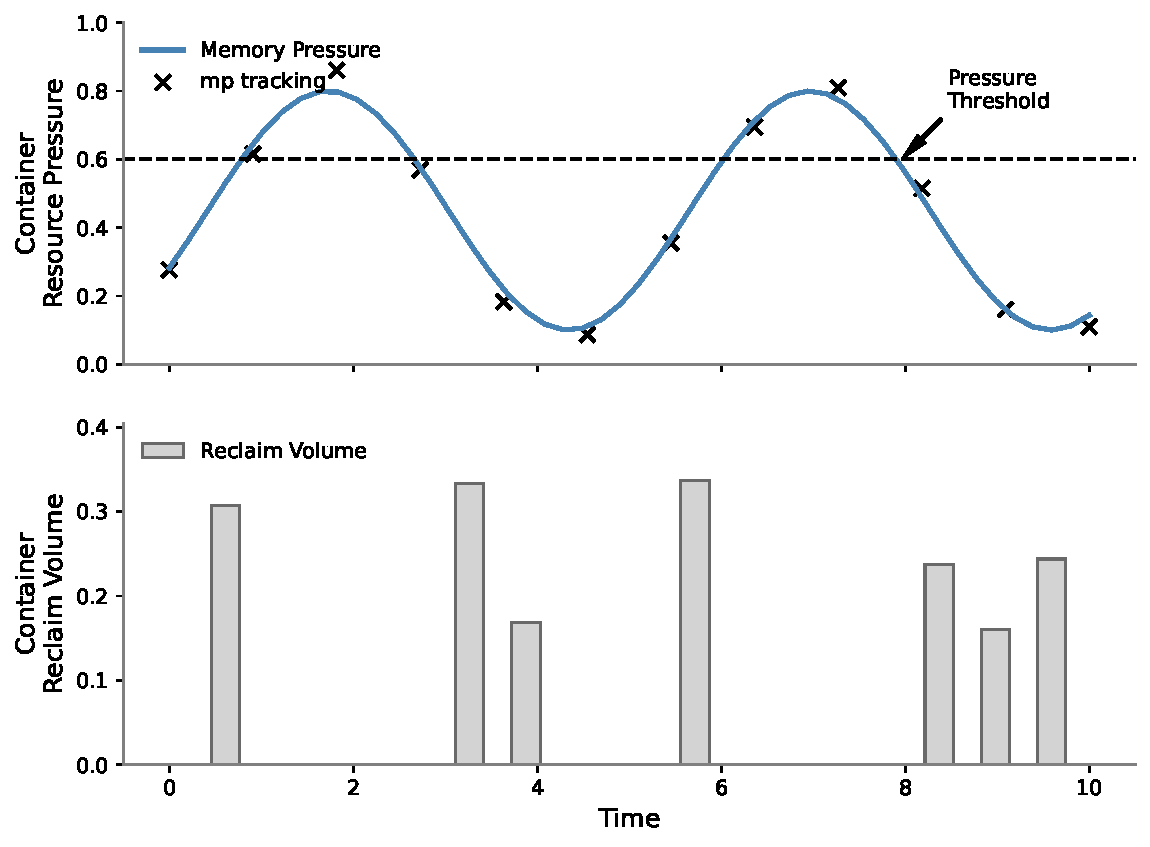
\includegraphics[width=0.95\textwidth]{压力与回收.pdf}
% % \caption{内存压力与页面回收调控机制}
% % \label{fig:pressure_work_set}
% % \end{figure}

% % 本算法通过压力量化与反馈机制来实现内存的动态调控。不同于传统的静态内存管理策略,本算法根据系统的实时内存压力调整内存的使用范围,确保系统在高负载时能够扩展内存资源,在低负载时又能将冷页面主动卸载。这种基于内存压力的调控方法能够有效应对突发负载变化,并在保证系统稳定性的同时,提高内存资源的利用率。

% % 图\ref{fig:pressure_work_set}展示了本模型的设计目标,即通过监控系统的内存压力,采用动态调整策略,确保系统内存处于合理的使用范围内。具体而言,当系统内存压力超过设定目标时,系统会逐步放宽内存限制;反之,内存压力较低时,系统会收紧内存限制。这样,不仅能在高负载时避免内存不足的问题,还能在低负载时将冷页面主动卸载。

% % 本算法采用基于压力负反馈机制,其中的关键参数体系如表\ref{tab:params}所示。算法每6秒钟执行一次,设定一个目标内存压力阈值,实现系统的平滑调节。压力误差是通过比较实际内存压力与目标内存压力阈值的差异来计算的,从而形成一个时间窗口内的压力累积效应。


% % \begin{table}[H]
% % \centering
% % \caption{调控参数体系}
% % \label{tab:params}
% % \begin{tabular}{cccc}
% % \toprule
% % 参数 & 符号 & 默认值 & 作用域 \\
% % \midrule
% % 目标压力 & \(mem\_pressure\_target\) & 0.1\% & 全局 \\
% % 最大收缩率 & \(M_p\) & 0.01 & 缩容阶段 \\
% % 最大扩张率 & \(M_b\) & 1.0 & 扩容阶段 \\
% % 收缩灵敏度 & \(C_p\) & 10 & 缩容触发 \\
% % 扩张灵敏度 & \(C_b\) & 20 & 扩容触发 \\
% % \bottomrule
% % \end{tabular}
% % \end{table}

% % \begin{algorithm}[H]
% %     \caption{基于压力的内存调控算法}
% %     \label{alg:control}
% %     \Input{\(mem\_pressure\), \(mem\_pressure\_target\), \(C_b\), \(C_p\), \(M_b\), \(M_p\), \(min\_size\), \(max\_size\)}
% %     \Output{Memory Limit \(Limit\)}
% %     \While{\textrm{true}}{  
% %         \(mem\_pressure\) get from proc file system;\\
% %         \If{\(mem\_pressure > mem\_pressure\_target\)}{
% %             % Calculate expansion coefficient eta
% %             \(\eta \leftarrow \min\left(\left(\frac{mem\_pressure/mem\_pressure\_target}{C_b}\right)^2, 1\right)\)*\(M_b\)\;
% %             % Perform expansion
% %             \(Limit \leftarrow \min(max\_size, Limit \times (1 + \eta))\)\;
% %             }
% %         \Else{
% %             % Calculate contraction coefficient eta
% %             \(\eta \leftarrow \min\left(\left(\frac{mem\_pressure\_target/mem\_pressure}{C_p}\right)^2, 1\right)\)*\(M_p\)\;
% %             % Perform contraction
% %             \(Limit \leftarrow \max(min\_size, Limit \times (1 - \eta))\)\;
% %             }
% %         % Apply the new memory limit
% %         Apply new memory limit \(Limit\)\;
% %     }
% % \end{algorithm}

% % \begin{itemize}
% % \item \textbf{灵敏度系数(\(C_p, C_b\))}: 
% %   \begin{itemize}
% %   \item 扩张灵敏度\(C_b=20\): 当累积压力超过目标值20倍时达到最大扩容比例
% %   \item 收缩灵敏度\(C_p=10\): 当压力低于目标值1/10时触发最大缩容
% %   \end{itemize}

% % \item \textbf{最大比例(\(M_p, M_b\))}: 
% %   \begin{itemize}
% %   \item \(M_b=1.0\)允许单次扩容100\%,应对突发压力
% %   \item \(M_p=0.01\)限制单次缩容1\%,确保服务稳定性
% %   \end{itemize}

% % \item \textbf{积分机制}: 
% %   \begin{itemize}
% %   \item 累积窗口\(T_{interval}=6s\)平滑瞬时波动
% %   \item 压力增量\(\Delta P\)累计检测持续负载
% %   \end{itemize}
% % \end{itemize}

% % 本算法的设计考虑了内存压力的动态变化与不同负载场景下的需求,因此参数体系中包含了多种灵敏度、最大收缩比例、扩张比例等调控因子,用于灵活应对系统的负载变化。例如,扩张灵敏度\(C_b = 20\)表示当实际内存压力超过目标压力的20倍时,系统会达到最大扩容比例;收缩灵敏度\(C_p = 10\)则表示当实际内存压力低于目标压力的1/10时,系统会触发最大缩容。

% % 最大扩张比例\(M_b = 1.0\)允许单次扩容至最大限制的100\%,应对突发的内存压力;而最大收缩比例\(M_p = 0.01\)限制单次缩容不超过1\%,确保系统的稳定性,避免因过快的收缩而导致服务质量下降。通过这些参数的调整,系统能够灵活应对不同的负载条件,避免内存资源的过度浪费,并确保在需要时能够快速扩展内存。


% % 需要特别强调的是,上述算法只是一个示例,目的是展示如何基于内存压力进行动态调控。在实际应用中,用户可以根据不同的QoS要求、系统负载特性或硬件架构,单独配置这些参数,甚至根据负载类型重新定义内存调控策略。例如,在某些高实时性应用中,可能会选择较高的扩张灵敏度 \(C_b\) 和较低的收缩灵敏度 \(C_p\),以确保快速响应压力变化。而在对于一般后台任务的处理上,则可能会选用较为保守的策略,以确保稳定性和节省资源。

% % 通过采用灵活配置的方式,本算法能够根据不同的需求调整内存压力阈值、调节因子和策略参数,从而提供更具针对性和适应性的内存管理策略。算法的灵活性使得它能够适用于不同的负载场景和硬件环境,满足各种不同应用的内存管理需求。

% % 此外,该算法可以结合不同的内存管理机制,如基于事件驱动的非阻塞方法,避免轮询带来的性能损失。未来也可以通过引入机器学习或预测算法,自动调整调控策略和参数,以实现更加智能和自适应的内存管理。算法本身也可以与其他资源管理策略结合,共同优化系统的整体性能和资源分配。



% % \section{基于内存压力的动态调控模型}
% % \label{sec:pressure_based_model}

% % 传统的工作集估计方法通常依赖于内存分配计数器、回收事件计数器等间接指标,这些方法的有效性受限于运维人员对存储硬件特性与内核行为的专业认知。在\ref{chap:基于同步内存回收的内存压力量化算法的设计与实现}中,本研究提出了基于同步内存回收的压力指标,该指标能够自适应不同的负载和异构卸载后端。本节基于定义的内存压力,实现了一种基于内存压力的动态调控模型。该模型采用主动回收策略,通过监控系统内存压力来维持目标压力区间,并将低访问频率的数据页迁移至基于 frontswap 的异构存储后端,从而实现内存利用率的优化。

% % \begin{figure}[h]
% % \centering
% % 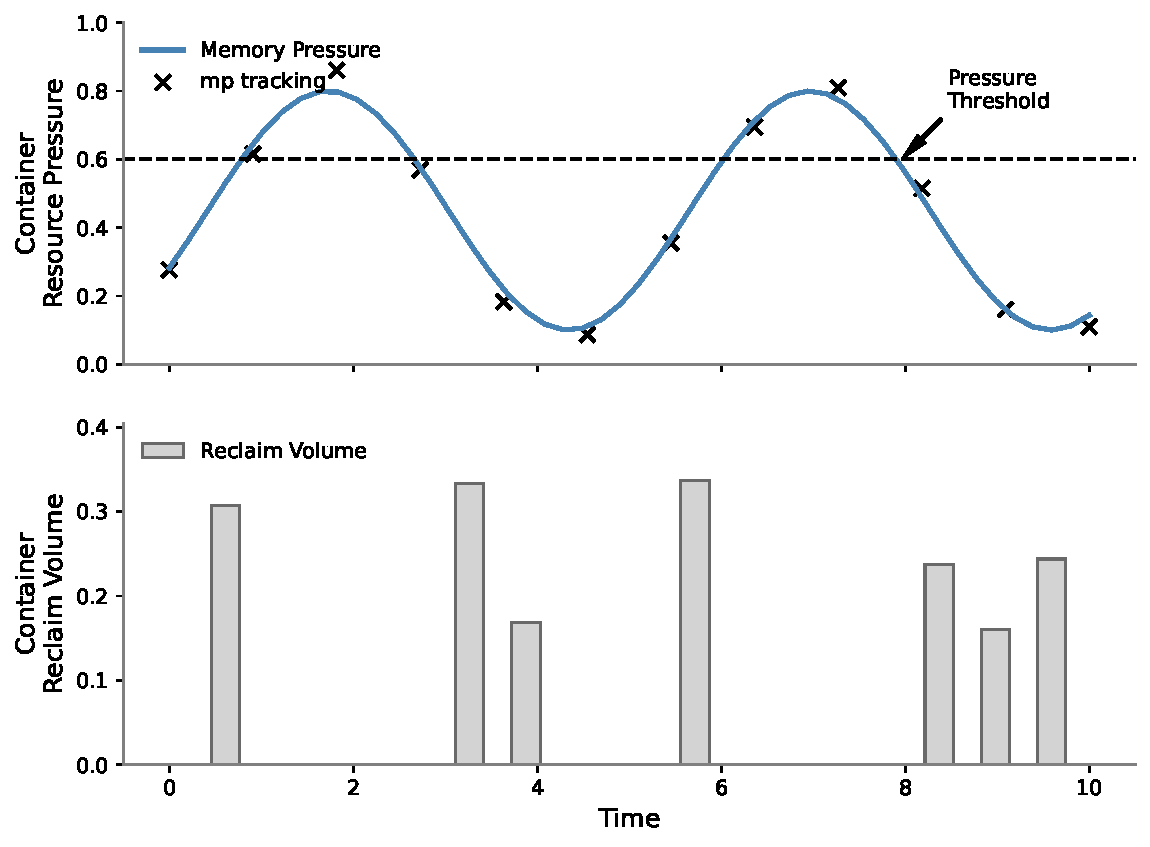
\includegraphics[width=0.95\textwidth]{压力与回收.pdf}
% % \caption{内存压力与页面回收调控机制}
% % \label{fig:pressure_work_set}
% % \end{figure}

% % 算法\ref{alg:control}通过压力量化与反馈机制实现内存的动态调控。与传统的静态内存管理策略不同,本算法根据系统的实时内存压力动态调整内存的使用范围,确保系统在高负载时能够扩展内存资源,在低负载时又能将冷页面主动卸载。这种基于内存压力的调控方法能够有效应对突发负载变化,在保证系统稳定性的同时,提高内存资源的利用率。

% % 图\ref{fig:pressure_work_set}展示了本模型的设计目标,即通过监控系统的内存压力,采用动态调整策略,确保系统内存处于合理的使用范围内。具体而言,当系统内存压力超过设定目标时,系统会逐步放宽内存限制;反之,当内存压力较低时,系统会收紧内存限制。这种机制不仅能够在高负载时避免内存不足的问题,还能在低负载时将冷页面主动卸载,从而提高内存资源的利用效率。

% % 本算法采用基于压力负反馈的调控机制,其关键参数体系如表\ref{tab:params}所示。算法每 6 秒钟执行一次,设定一个目标内存压力阈值,实现系统的平滑调节。压力误差通过比较实际内存压力与目标内存压力阈值的差异来计算,从而形成一个时间窗口内的压力累积效应。

% % 在算法中,灵敏度系数 \(C_p\) 和 \(C_b\) 分别用于控制收缩和扩张的触发条件。扩张灵敏度 \(C_b = 20\) 表示当累积压力超过目标值 20 倍时,系统会达到最大扩容比例;收缩灵敏度 \(C_p = 10\) 表示当压力低于目标值 1/10 时,系统会触发最大缩容。最大扩张比例 \(M_b = 1.0\) 允许单次扩容至最大限制的 100\%,以应对突发的内存压力;而最大收缩比例 \(M_p = 0.01\) 限制单次缩容不超过 1\%,确保系统的稳定性,避免因过快的收缩而导致服务质量下降。

% % \begin{table}[H]
% % \centering
% % \caption{调控参数体系}
% % \label{tab:params}
% % \begin{tabular}{cccc}
% % \toprule
% % 参数 & 符号 & 默认值 & 作用域 \\
% % \midrule
% % 目标压力 & \(mem\_pressure\_target\) & 0.1\% & 全局 \\
% % 最大收缩率 & \(M_p\) & 0.01 & 缩容阶段 \\
% % 最大扩张率 & \(M_b\) & 1.0 & 扩容阶段 \\
% % 收缩灵敏度 & \(C_p\) & 10 & 缩容触发 \\
% % 扩张灵敏度 & \(C_b\) & 20 & 扩容触发 \\
% % \bottomrule
% % \end{tabular}
% % \end{table}



% % \begin{algorithm}[H]
% %     \caption{基于压力的内存调控算法}
% %     \label{alg:control}
% %     \Input{\(mem\_pressure\), \(mem\_pressure\_target\), \(C_b\), \(C_p\), \(M_b\), \(M_p\), \(min\_size\), \(max\_size\)}
% %     \Output{Memory Limit \(Limit\)}
% %     \While{\textrm{true}}{
% %         \(mem\_pressure\) get from proc file system;\\
% %         \If{\(mem\_pressure > mem\_pressure\_target\)}{
% %             \(\eta \leftarrow \min\left(\left(\frac{mem\_pressure/mem\_pressure\_target}{C_b}\right)^2, 1\right)\)*\(M_b\)\;
% %             \(Limit \leftarrow \min(max\_size, Limit \times (1 + \eta))\)\;
% %             }
% %         \Else{
% %             \(\eta \leftarrow \min\left(\left(\frac{mem\_pressure\_target/mem\_pressure}{C_p}\right)^2, 1\right)\)*\(M_p\)\;
% %             \(Limit \leftarrow \max(min\_size, Limit \times (1 - \eta))\)\;
% %             }
% %         Apply new memory limit \(Limit\)\;
% %     }
% % \end{algorithm}

% % 此外,算法通过积分机制平滑瞬时波动,累积窗口 \(T_{interval} = 6s\) 用于检测持续负载,压力增量 \(\Delta P\) 用于累计压力变化。这种设计使得算法能够灵活应对不同的负载条件,避免内存资源的过度浪费,并确保在需要时能够快速扩展内存。

% % 需要特别强调的是,上述算法只是一个示例,目的是展示如何基于内存压力进行动态调控。在实际应用中,用户可以根据不同的 QoS 要求、系统负载特性或硬件架构,单独配置这些参数,甚至根据负载类型重新定义内存调控策略。例如,在某些高实时性应用中,可能会选择较高的扩张灵敏度 \(C_b\) 和较低的收缩灵敏度 \(C_p\),以确保快速响应压力变化;而在一般后台任务的处理上,则可能会选用较为保守的策略,以确保稳定性和节省资源。

% % 通过采用灵活配置的方式,本算法能够根据不同的需求调整内存压力阈值、调节因子和策略参数,从而提供更具针对性和适应性的内存管理策略。算法的灵活性使得它能够适用于不同的负载场景和硬件环境,满足各种不同应用的内存管理需求。

% % 此外,该算法可以结合不同的内存管理机制,如基于事件驱动的非阻塞方法,避免轮询带来的性能损失。未来也可以通过引入机器学习或预测算法,自动调整调控策略和参数,以实现更加智能和自适应的内存管理。算法本身也可以与其他资源管理策略结合,共同优化系统的整体性能和资源分配。
% \section{基于内存压力的动态调控模型}
% \label{sec:pressure_based_model}

% 传统的工作集估计方法主要依赖于内存分配计数器、回收事件计数器等间接指标,这些方法的有效性受限于对存储硬件特性与内核行为的专业认知要求。为解决这一问题,\ref{chap:基于同步内存回收的内存压力量化算法的设计与实现}章节提出了基于同步内存回收的压力指标,该指标对不同负载类型和异构卸载后端具有普适性。本节在此基础上,构建了一种基于内存压力的动态调控模型。该模型通过持续监测系统内存压力指标,实施主动回收策略,将低访问频率的数据页迁移至基于frontswap的异构存储后端,从而在保证系统性能的前提下优化内存资源利用率。

% \begin{figure}[h]
% \centering
% 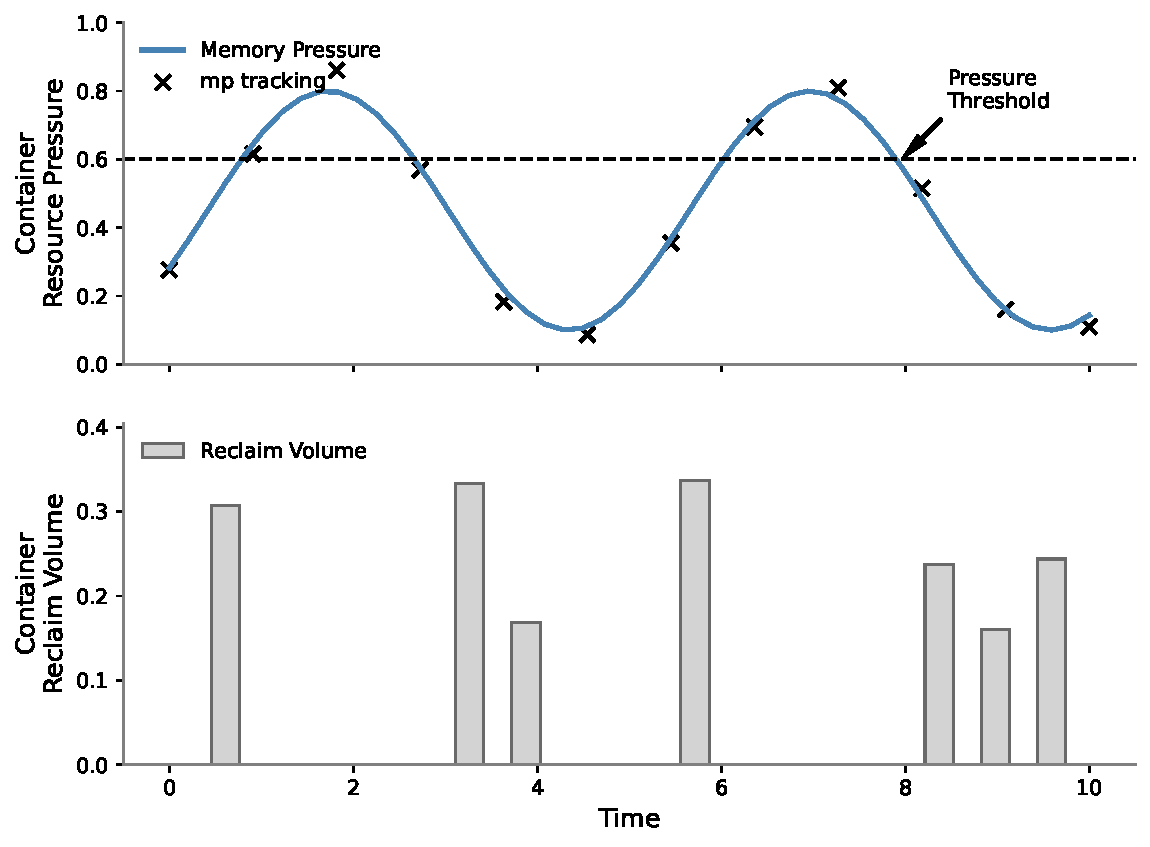
\includegraphics[width=0.95\textwidth]{压力与回收.pdf}
% \caption{内存压力与页面回收调控机制}
% \label{fig:pressure_work_set}
% \end{figure}

% 图\ref{fig:pressure_work_set}展示了本模型的核心设计目标及运行机制。通过建立一个压力感知的闭环调控系统,该模型能够根据测量的内存压力值动态调整内存使用边界。当系统内存压力超过预设阈值时,模型逐步放宽内存限制以应对增长的工作集需求;反之,当内存压力低于目标值时,模型主动收紧内存限制并触发冷页面卸载,从而释放未充分利用的内存资源。这种基于压力的负反馈机制确保系统能够在不同负载条件下维持接近最优的内存分配状态。

% 算法\ref{alg:control}详细描述了基于压力量化的动态调控机制。与传统的静态内存分配策略不同,该算法通过实时内存压力指标构建了资源分配的动态反馈系统。算法以固定的时间间隔(默认6秒)执行一次评估,通过计算当前内存压力与目标压力阈值间的偏差来确定调整策略和幅度。

% \begin{table}[H]
% \centering
% \caption{调控参数体系}
% \label{tab:params}
% \begin{tabular}{cccc}
% \toprule
% 参数 & 符号 & 默认值 & 作用域 \\
% \midrule
% 目标压力 & \(mem\_pressure\_target\) & 0.1\% & 全局 \\
% 最大收缩率 & \(M_p\) & 0.01 & 缩容阶段 \\
% 最大扩张率 & \(M_b\) & 1.0 & 扩容阶段 \\
% 收缩灵敏度 & \(C_p\) & 10 & 缩容触发 \\
% 扩张灵敏度 & \(C_b\) & 20 & 扩容触发 \\
% \bottomrule
% \end{tabular}
% \end{table}

% 表\ref{tab:params}列出了算法的关键参数体系。目标压力值(\(mem\_pressure\_target\))作为全局调控基准,默认设置为0.1\%,表示系统期望维持的同步回收延迟占比。灵敏度系数(\(C_p\)和\(C_b\))控制系统对压力变化的响应程度:扩张灵敏度\(C_b = 20\)表示当实际压力达到目标值20倍时,触发最大扩容比例;收缩灵敏度\(C_p = 10\)表示当压力降至目标值1/10时,系统执行最大缩容操作。最大调整率参数(\(M_b\)和\(M_p\))限定了单次调整的幅度上限:最大扩张比例\(M_b = 1.0\)允许在单次调整中将内存限制扩大至原值的两倍,以快速响应突发性工作负载;最大收缩比例\(M_p = 0.01\)将单次缩容限制在1%以内,确保系统稳定性并避免服务质量剧烈波动。

% \begin{algorithm}[H]
%     \caption{基于压力的内存调控算法}
%     \label{alg:control}
%     \Input{\(mem\_pressure\), \(mem\_pressure\_target\), \(C_b\), \(C_p\), \(M_b\), \(M_p\), \(min\_size\), \(max\_size\)}
%     \Output{Memory Limit \(Limit\)}
%     \While{\textrm{true}}{
%         \(mem\_pressure\) get from proc file system;\\
%         \If{\(mem\_pressure > mem\_pressure\_target\)}{
%             \(\eta \leftarrow \min\left(\left(\frac{mem\_pressure/mem\_pressure\_target}{C_b}\right)^2, 1\right)\)*\(M_b\)\;
%             \(Limit \leftarrow \min(max\_size, Limit \times (1 + \eta))\)\;
%             }
%         \Else{
%             \(\eta \leftarrow \min\left(\left(\frac{mem\_pressure\_target/mem\_pressure}{C_p}\right)^2, 1\right)\)*\(M_p\)\;
%             \(Limit \leftarrow \max(min\_size, Limit \times (1 - \eta))\)\;
%             }
%         Apply new memory limit \(Limit\)\;
%     }
% \end{algorithm}

% 算法通过二次函数映射将压力偏差转换为调整系数,采用平方关系确保对小偏差具有较低敏感度,而对大偏差则产生更强响应。这种设计避免了因瞬时波动导致的频繁调整,同时保证了对持续性压力变化的及时响应。算法还通过积分机制累积一定时间窗口内的压力变化,以检测持续性负载趋势而非瞬时波动,进一步提高了系统稳定性。

% 需要强调的是,上述算法设计具有高度可配置性,允许根据不同应用场景和性能需求进行参数调整。在高实时性要求的环境中,可以配置较高的扩张灵敏度和较低的收缩灵敏度,实现对压力增长的快速响应;而在资源受限且对性能波动容忍度较高的场景中,则可采用更积极的收缩策略以最大化资源利用率。通过这种参数化设计,算法能够适应从延迟敏感型在线服务到吞吐量导向的批处理任务等各类工作负载特性。

% 此调控模型的优势在于将内存管理决策建立在直接测量的系统压力之上,而非依赖难以精确估计的工作集大小。这种方法既避免了传统启发式算法在异构系统上的适应性问题,又实现了对资源利用的精细调控。未来研究方向包括引入机器学习技术实现参数的自适应调整,以及将该模型扩展至更广泛的资源管理领域,如CPU、IO带宽等多维资源的协同优化。


% \section{基于重用距离的自适应页面回收策略}
% \label{sec:基于重用距离的冷热页面优化}

% \subsection{重用距离}

% 设计一种通用的、高效的冷热页面识别算法具有挑战性,人们通过分析负载的特征来提出启发式的算法。Linux很早就提出了基于重用距离(Reuse Distance)\citing{jiang2002lirs,jiang2005clockpro}的冷热页面识别,但是该算法落地困难,需要额外的辅助信息来实现。本研究将其引入页面替换策略的设计,以在文件页面与匿名页面的回收之间取得更佳平衡。重用距离刻画某一页面两次访问之间,被访问过的不同页面的数量,能在一定程度上反映页面的访问模式及其在替换时的优先级。

% 对一段内存访问序列
% \[
%   A \;=\;\{\,a_1,\,a_2,\,\dots,\,a_n\},
% \]
% 其中 \(a_i\) 表示第 \(i\) 次访问的页面。令 \(P\) 为所关心的目标页面,则可将其重用距离定义为
% \begin{align}
% \label{eq:rd_def}
%   RD(P) 
%   &= 
%   \min\Bigl\{\,j - i
%     \;\Bigm|\;
%     a_i = P,\;
%     a_j = P,\;
%     i < j
%   \Bigr\}.
% \end{align}


% 页面的重用距离与其访问频率密切相关。直观而言,若 \(RD(P)\)  较短,则表明页面  \(P\) 在近期被频繁访问,具有较高的局部性;若  \(P\) 较长,则表明其访问稀疏,通常可作为回收候选。

% \begin{figure}[htbp]
%   \centering
%   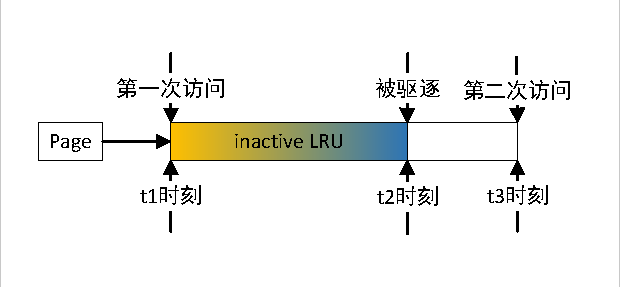
\includegraphics[width=0.5\textwidth]{重用距离.pdf}
%   \caption{重用距离示意图}
%   \label{fig:refault_distance}
% \end{figure}

% 如图 \ref{fig:refault_distance} 所示,页面的重用距离就是t1到t3时间段内,访问过的不同页面的数量。通过分析页面重用距离的分布,可以识别出访问模式,从而及时调整页面替换策略。然而,在大型系统中精确计算每个页面的重用距离会引入显著的空间开销和计算开销。为此,本研究提出了一种基于页面在活动链表和非活动链表间迁移行为的近似策略,通过观察页面在链表中的位置变化来间接推断其访问频度。当页面在非活动链表上被替换(即被驱逐)时,如果它在短期内再次被访问(即发生refault),则说明在两次访问之间,系统至少经历了与非活动链表长度相当数量的页面访问。因此,可以通过统计refault的次数和间隔来近似估计页面的访问频率。


% \subsection{重用距离的近似推导}

% 为了简化分析,先假设非活动链表长度固定,且暂不考虑活动链表向非活动链表的降级。这样可以更直观地专注于非活动链表上的页面替换与访问。图 \ref{fig:现象1} 与图 \ref{fig:现象2} 展示了两种核心场景。

% \begin{figure}[htbp]
%   \centering
%   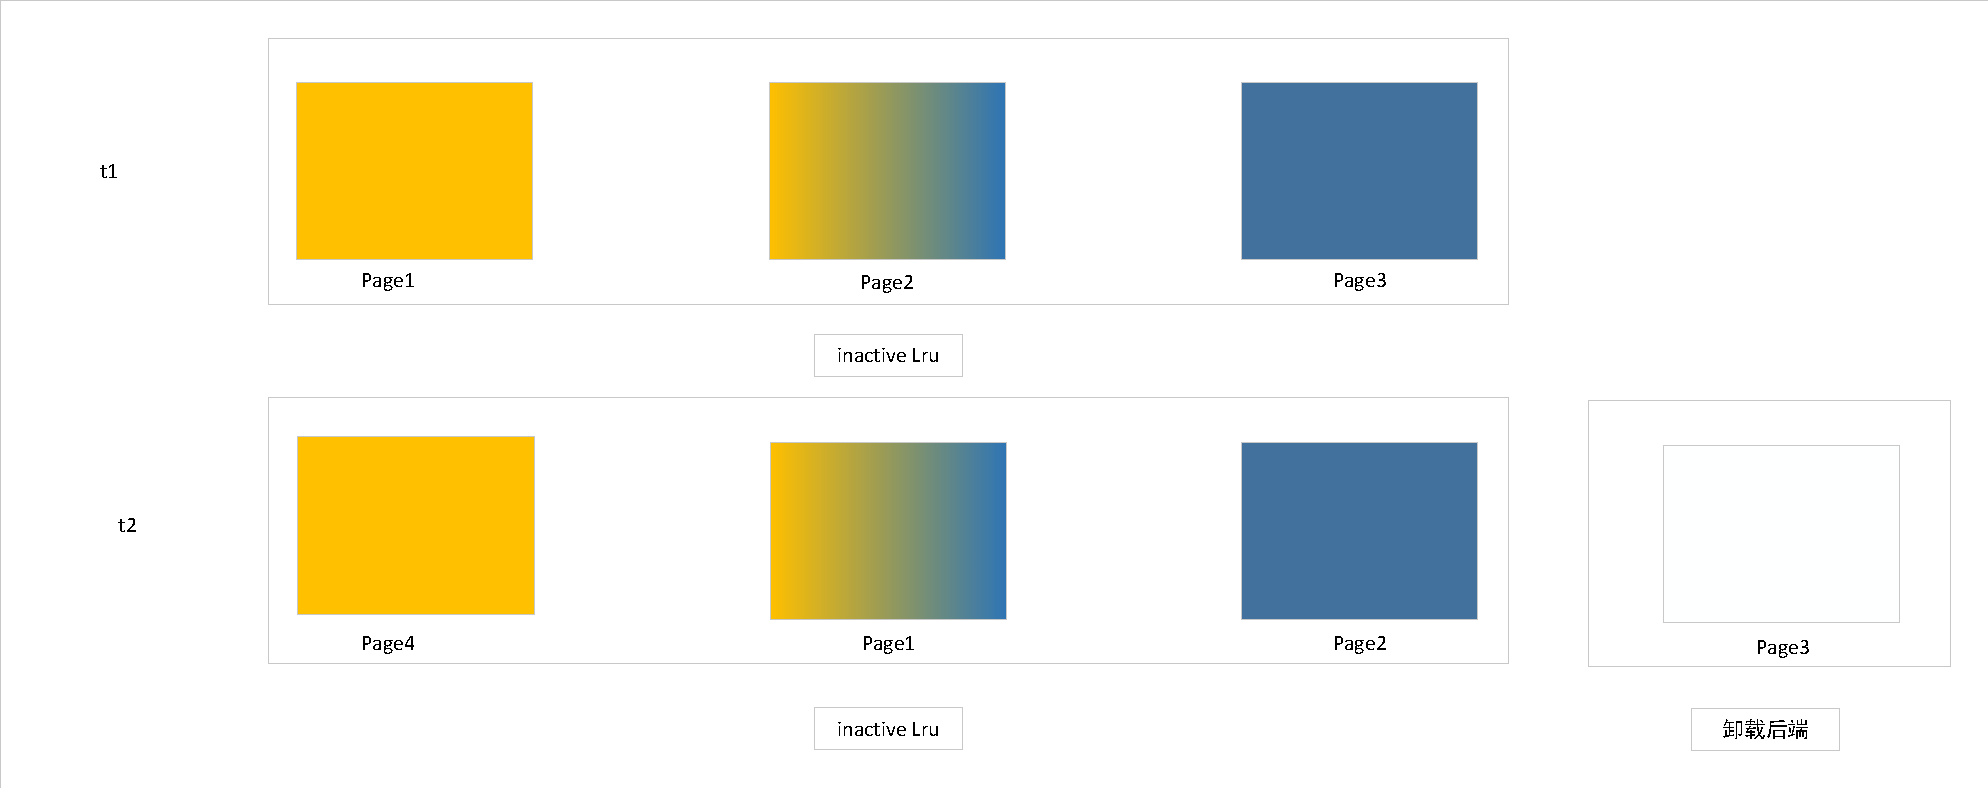
\includegraphics[width=0.5\textwidth]{现象1.pdf}
%   \caption{页面首次插入非活动链表}
%   \label{fig:现象1}
% \end{figure}

% \begin{figure}[htbp]
%   \centering
%   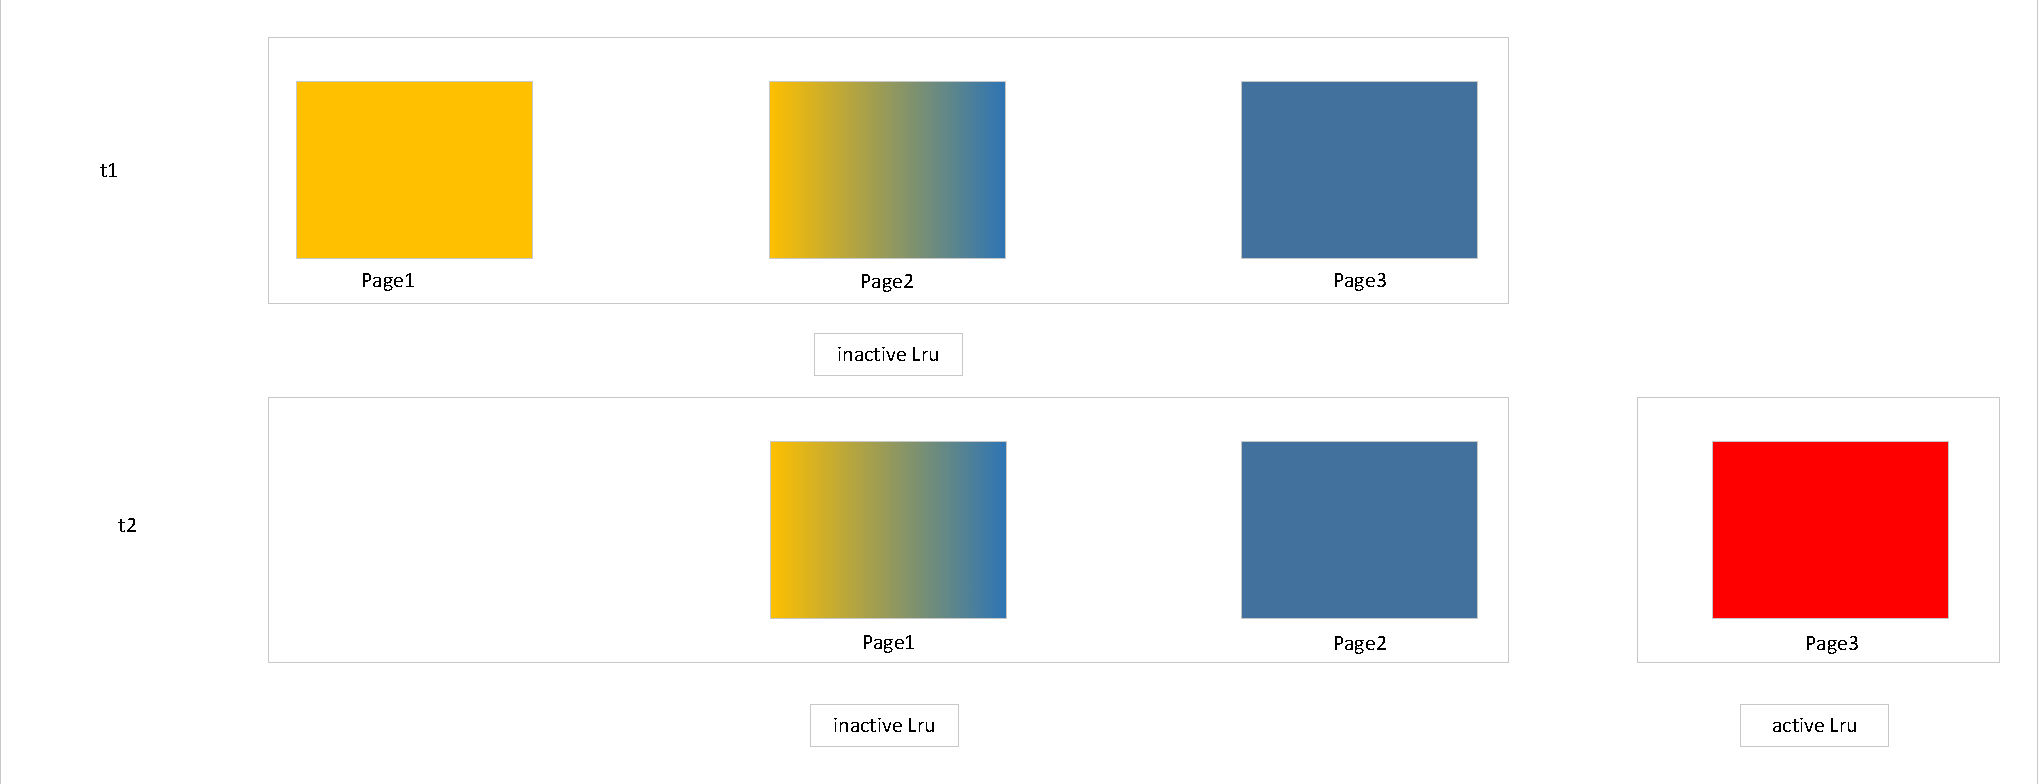
\includegraphics[width=0.5\textwidth]{现象2.pdf}
%   \caption{页面在非活动链表上再次被访问并提升到活动链表}
%   \label{fig:现象2}
% \end{figure}

% \noindent
% \textbf{情形一}(图 \ref{fig:现象1})描述页面首次被访问并插入到非活动链表头部;由于链表长度固定,原链表中的页面整体向尾部滑动,最末尾页面被挤出内存(驱逐)。  
% \textbf{情形二}(图 \ref{fig:现象2})描述页面在非活动链表上再次被访问后,被提升到活动链表,链表长度相应缩短;与此同时,所有比被提升页面更晚进入非活动链表的页面向尾部滑动,离被驱逐更近。

% 在时间区间 \([t_1, t_2]\) 内,非活动链表上的页面要么被驱逐(表明至少加载了新的页面),要么被提升至活动链表(表明被再次访问)。令
% \(
%   E(t_1,t_2)
% \)
% 表示该区间内的驱逐次数,令
% \(
%   A(t_1,t_2)
% \)
% 表示该区间的页面提升次数。因为每次驱逐对应至少一次新页面的载入,每次提升对应至少一次对非活动链表中页面的访问,故可以近似认为 \([t_1,t_2]\) 时间段内发生的最少页面访问数不低于
% \(
%   E(t_1,t_2) \;+\; A(t_1,t_2).
% \)
% 。真实系统中还需考虑一直停留在活动链表、从未降级的页面访问量。不过,对访问极频繁的页面而言,由于它们并不进入非活动链表,无需担心其再次访问情形的遗漏,因此对这部分页面的统计影响相对有限。

% 当页面 $p$ 被驱逐时,记录其驱逐时刻 $t_1$ 对应的全局计数器 $\mathrm{count}(t_1)$,该计数器累积了系统自启动以来的总驱逐次数和提升次数。

% 若该页面于时刻 \(t_2\) 再次被访问,则同样记录 \(count(t_2)\)。此时,基于上述计数器,定义页面 \(p\) 的重用距离(Refault Distance)为
% \begin{align}
%   \label{eq:refault_distance}
%   RD_{\mathrm{refault}}(p)
%   &= 
%   \mathrm{count}(t_2)
%   \;-\;
%   \mathrm{count}(t_1).
% \end{align}
% 这一距离衡量了页面从被驱逐到再次访问期间,系统所经历的最少页面访问次数。

% 由于页面在非活动链表中从头部移动到尾部直至被驱逐的过程,可以近似看作是经历了一系列其他页面的访问,因此,非活动链表的长度 $L_{\mathrm{inactive}}$ 可以作为页面在缓存中停留期间所经历的页面访问次数的估计。综合考虑页面在非活动链表中的移动和refault期间的访问,则可得到页面 \(p\) 的总访问距离近似形式:
% \begin{align}
%   \label{eq:dtotal}
%   RD_{\mathrm{total}}(p)
%   &= 
%   L_{\mathrm{inactive}}
%   \;+\;
%   \bigl(\mathrm{count}(t_2) \;-\; \mathrm{count}(t_1)\bigr).
% \end{align}


% 当非活动链表长度较小时,$\mathrm{count}(t_2) - \mathrm{count}(t_1)$ 的增量会相对较大,这表明页面需要具有更高的访问频率才能在非活动链表中停留足够长的时间而不被快速驱逐。

% \subsection{替换决策与回收策略}

% 为了确定页面是否应该继续保留在内存中,需要综合考虑其在非活动链表中的重用距离和活动链表的长度。
% \begin{align}
%   \label{eq:active_condition_1}
%   L_{\mathrm{inactive}}
%   \;+\;
%   \bigl(\mathrm{count}(t_2) \;-\; \mathrm{count}(t_1)\bigr)
%   &\;\;\le\;\;
%   L_{\mathrm{inactive}}
%   \;+\;
%   L_{\mathrm{active}}
% \end{align}
% 化简后即
% \begin{align}
%   \label{eq:active_condition}
%   \mathrm{count}(t_2) - \mathrm{count}(t_1)
%   \;\le\;
%   L_{\mathrm{active}}
% \end{align}

% 由此可知,当页面的重用距离不超过活动链表大小时,该页面的访问频度足以支撑其继续驻留在内存,避免被替换。

% 在Linux内核中,可以将该方法与操作系统中的 \(\mathrm{swappiness}\) 等超参数结合,动态调整文件页与匿名页的回收策略。例如,
% \begin{equation}
%   \label{swappiness1}
%   \mathrm{swappiness} = \min \left( \mathrm{swappiness} \times (1 + \mathrm{refault\_active}), \; 150 \right)
% \end{equation}  

% 其中 \(\mathrm{refault\_active}\) 代表在近一段时间内页面重新故障的比例,通过该值对回收过程进行调节。当系统检测到高refault率时,表明当前回收策略过于激进,可能错误地驱逐了热页面,此时应适当增加$\mathrm{swappiness}$ 值以提高文件页的保留优先级;反之,当refault率较低时,可以适当减小 $\mathrm{swappiness}$ 值以加速匿名页的回收。

% 综上所述,本文提出的基于重用距离近似估计的页面替换策略,能够在较低开销下有效识别冷热页面,并指导文件页和匿名页的回收决策,从而提高内存利用率和系统整体性能。


% \subsection{基于阴影条目的重用距离实现}

% 前文提出的基于重用距离的冷热页面优化算法,需要在内核中实现多个关键机制以支持其运行。本节将从全局计数维护、页面驱逐与再加载的处理流程以阴影条目的复用三个方面,详细阐述该算法在内核中的实现原理与机制。

% \subsubsection{全局计数维护}

% 为了实现基于重用距离的页面替换策略,需要在内核中维护以下关键计数信息:

% \begin{enumerate}
%   \item 全局的驱逐和提升次数之和(记为 \(\mathrm{nr\_count}\))
%   \item 上次重新故障统计的次数之和(记为 \(\mathrm{nr\_refault\_last}\))
%   \item 当前时刻累积的重新故障次数之和(记为 \(\mathrm{nr\_refault}\))
%   \item 文件页面被驱逐时对应的驱逐与提升次数之和
% \end{enumerate}

% 其中,前三项计数直接存储在 lruvec 结构体的原子变量中。每当页面发生驱逐或提升事件时,为了保证并发访问时的计数准确性,需要对 $\mathrm{nr\_count}$ 执行原子加一操作。当页面再次加载时,如果满足算法\ref{eq:active_condition}的条件,则表明该页面在被驱逐后不久即被再次访问,此时系统会将其视为一次 refault ,并相应地增加 \(\mathrm{nr\_refault}\) 计数。通过计算 $\mathrm{nr\_refault}$ 和 $\mathrm{nr\_refault\_last}$ 的差值,可以动态评估文件页的\(\mathrm{refault\_active}\),进而通过算法\ref{swappiness1}调整文件页和匿名页的回收比例。

% \subsubsection{阴影条目管理}

% Linux 内核中的 page cache 使用前缀树(Radix Tree)作为索引结构,通过文件偏移量来查找对应的 struct page 指针。图\ref{fig:前缀树}展示了通过前缀树查找文件偏移量为2222的页面在page cache中的对应项,每级节点根据页偏移量的特定位段进行寻址。前缀树通过路径压缩等优化技术,能够在节点分布稀疏的情况下有效降低内存占用。形式化地,第$i$级节点的选择可表示为:
% \[
% \text{node}_i = \text{node}_{i-1}.\text{slots}[(p_{\text{off}} \gg \text{shift}_i) \& \text{MASK}]
% \]

% 其中 $\text{node}_i$ 表示第 $i$ 级节点,$\text{node}_{i-1}$ 表示其父节点,$\text{slots}$ 表示节点中的槽位数组,$p_{\text{off}}$ 表示页偏移量,$\text{shift}_i$ 表示第 $i$ 级节点的位移量,$\text{MASK}$ 是一个位掩码常量,用于提取页偏移量中的相关位段。

% \begin{figure}[htbp]
%   \centering
%   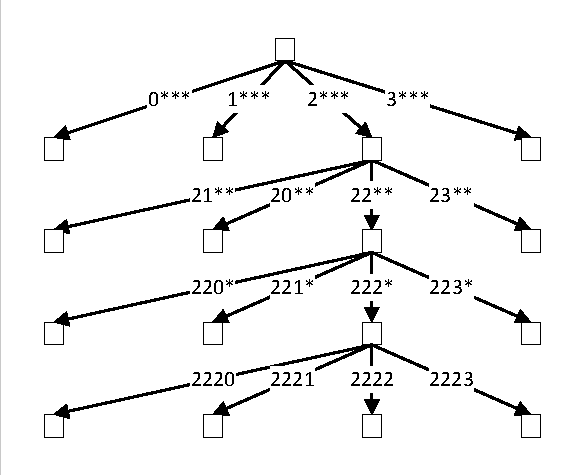
\includegraphics[width=\textwidth]{前缀树.pdf}
%   \caption{page cache 的前缀树结构示意}
%   \label{fig:前缀树}
% \end{figure}

% 最终得到的值是 struct page 的指针。为了节省内存空间,struct page 数据结构采用了紧凑的内存布局,并实现了16字节对齐所以指针的最后4位全是0。因此内核使用struct page 指针的后两位作为标识符。表\ref{tab:标志位}详细说明了这些标志位的含义与用途。为了实现页面被驱逐时记录全局计数的需求,系统复用了前缀树指针槽的标志位。

% \begin{table}[htbp]
%   \centering
%   \caption{struct page指针低两位标志位含义}
%   \label{tab:标志位}
%   \begin{tabular}{cc}
%     \toprule
%     \textbf{标志位} & \textbf{说明} \\
%     \midrule
%     \texttt{00} & 指向 \texttt{struct page} 的正常指针 \\
%     \texttt{01} & 内部节点 \\
%     \texttt{10} & 阴影条目(shadow entry) \\
%     \texttt{11} & 保留 \\
%     \bottomrule
%   \end{tabular}
% \end{table}

% 在 \_\_remove\_mapping 函数中,当文件页面即将被从page cache中移除时,系统执行以下步骤:

% \begin{enumerate}
%   \item 读取当前全局计数器 $\mathrm{nr\_count}$ 的值,并将其左移两位,为标志位预留空间。
%   \item 将移位后的计数器值与 $\texttt{10}$ 进行按位或运算,生成阴影条目,并将其写回前缀树的对应槽位。
%   \item 对全局计数器 $\mathrm{nr\_count}$ 进行原子递增操作,表示发生了一次页面驱逐。
%   \item 将页面从活动链表或非活动链表中移除,完成驱逐过程。
% \end{enumerate}

% 当后续对同一文件偏移发生缺页中断(page fault)而需要载入页面时,系统执行以下步骤:

% \begin{enumerate}
%   \item 内核检测到前缀树对应槽位存储的指针标志位不是 $\texttt{00}$,判断其为阴影条目。
%   \item 提取阴影条目中的数值,并将其右移两位,得到页面被驱逐时的全局计数器值 $\mathrm{count}(t_1)$。
%   \item 计算当前全局计数器值 $\mathrm{count}(t_2)$ 与 $\mathrm{count}(t_1)$ 的差值,如果该差值不超过活动链表长度 $L_{\mathrm{active}}$,则认为该页面在短期内被再次访问,将其提升至活动链表,并对 $\mathrm{nr\_refault}$ 计数器进行原子递增操作。
%   \item 如果差值超过 $L_{\mathrm{active}}$,则仅将该页面添加到非活动链表,不更新 $\mathrm{nr\_refault}$ 计数器。
% \end{enumerate}

% 如图 \ref{fig:复用} 所示,页面在内存中时使用普通指针(标志位 \texttt{00});被驱逐后则切换为阴影条目(标志位 \texttt{10});再加载时可根据此信息计算重用距离并作相应处理。该方法避免了在 \texttt{struct page} 内部额外存储驱逐计数,最大化复用内核已有数据结构。

% \begin{figure}[htbp]
%   \centering
%   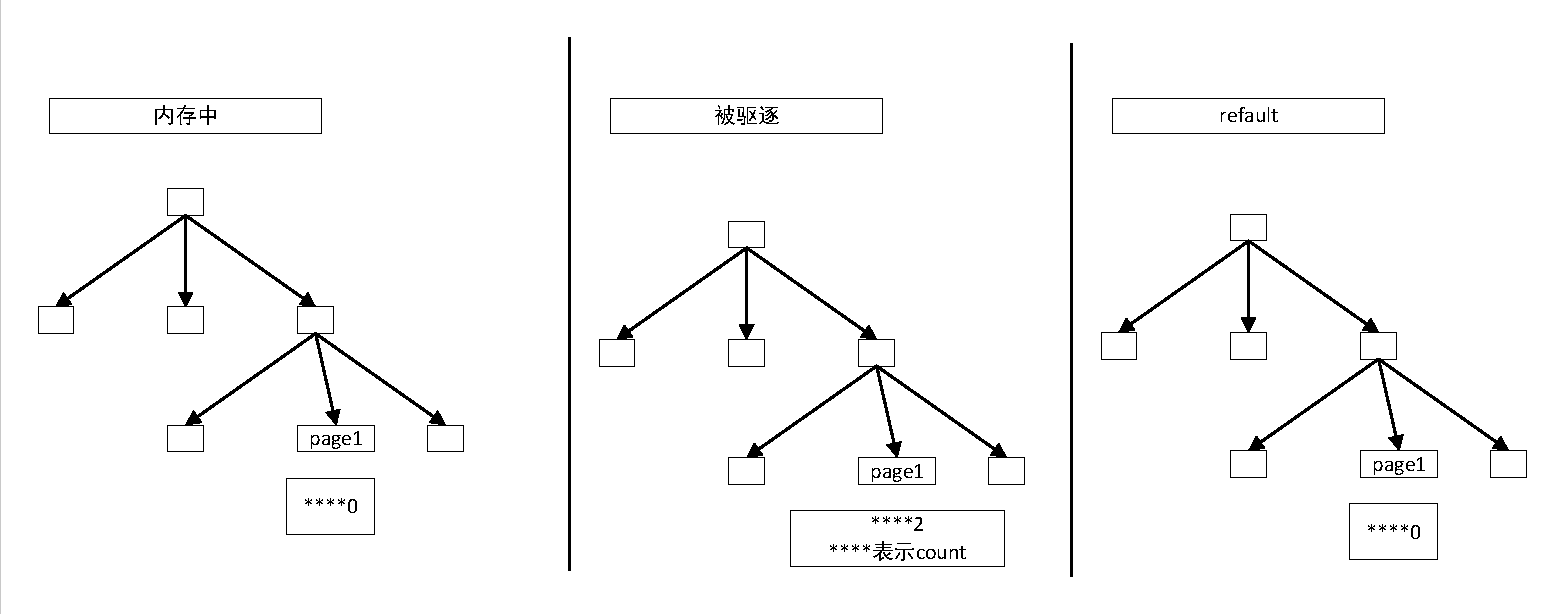
\includegraphics[width=\textwidth]{复用.pdf}
%   \caption{利用阴影条目存储驱逐时的 \(\mathrm{nr\_count}\)}
%   \label{fig:复用}
% \end{figure}



% \subsubsection{Shrinker回收机制}

% 在上一节中,我们介绍了如何通过复用前缀树指针的低位标志位来存储页面驱逐时的全局计数器值。然而,这种方法会导致前缀树中的阴影条目数量不断累积。如果不及时清理这些阴影条目,可能会导致前缀树过度膨胀,占用过多的内存资源。

% 为了解决阴影条目累积导致的内存浪费问题,本研究利用Linux内核提供的Shrinker机制来实现对阴影条目的自动回收。Shrinker 是 Linux 内核内存回收子系统中的统一回调接口,用于管理诸如 inode、dentry 等自定义缓存。

% Shrinker 通过 struct shrink\_control(表 \ref{tab:shrink_control_struct})与 struct shrinker(表 \ref{tab:shrinker_struct})两个核心数据结构向回收框架注册接口,内核则在内存压力情形下调用对应的回调函数执行清理动作。

% \begin{table}[htbp]
%   \centering
%   \caption{struct shrink\_control 结构体主要字段说明}
%   \label{tab:shrink_control_struct}
%   \begin{tabular}{ccc}
%     \toprule
%     \textbf{成员} & \textbf{类型} & \textbf{说明} \\
%     \midrule
%     \texttt{gfp\_mask} & \texttt{gfp\_t} & 本次内存分配的掩码,指示约束条件 \\
%     \texttt{nid} & \texttt{int} & 所在的 NUMA 节点 \\
%     \texttt{nr\_to\_scan} & \texttt{unsigned long} & 期望本轮扫描并回收的对象数 \\
%     \texttt{nr\_scanned} & \texttt{unsigned long} & 实际扫描对象数量 \\
%     \texttt{memcg} & \texttt{struct mem\_cgroup *} & 针对特定 \texttt{memcg} 的回收(若有) \\
%     \bottomrule
%   \end{tabular}
% \end{table}

% \begin{table}[htbp]
%   \centering
%   \caption{struct shrinker 结构体主要字段说明}
%   \label{tab:shrinker_struct}
%   \begin{tabular}{ccc}
%     \toprule
%     \textbf{成员} & \textbf{类型} & \textbf{说明} \\
%     \midrule
%     \texttt{count\_objects} & 函数指针 & 返回可回收对象数,若无可回收则 \texttt{SHRINK\_EMPTY} \\
%     \texttt{scan\_objects} & 函数指针 & 实际扫描并回收对象,返回已释放数量 \\
%     \texttt{batch} & \texttt{long} & 每次回收的批次大小,默认为 0(使用默认值) \\
%     \texttt{seeks} & \texttt{int} & 反映对象重建开销,影响回收优先级 \\
%     \texttt{flags} & \texttt{unsigned} & Shrinker 能力标志(NUMA 感知等) \\
%     \texttt{list} & \texttt{struct list\_head} & 内核内部使用,用于将 shrinker 链接到全局列表 \\
%     \texttt{id} & \texttt{int} & 在 memcg 上下文中的 shrinker 标识 \\
%     \texttt{nr\_deferred} & \texttt{atomic\_long\_t *} & 延迟对象数计数 \\
%     \bottomrule
%   \end{tabular}
% \end{table}

% \begin{figure}[htbp]
%   \centering
%   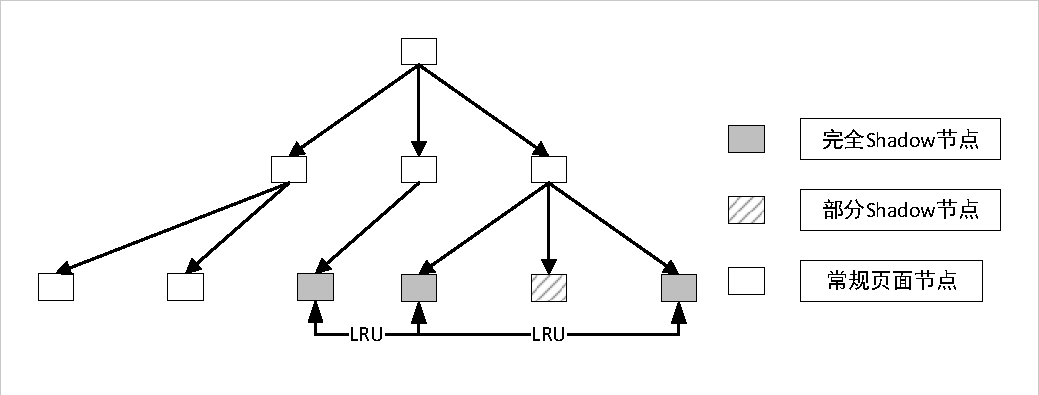
\includegraphics[width=\textwidth]{Shrinker设计.pdf}
%   \caption{Shrinker机制工作原理示意图}
%   \label{fig:shrink}
% \end{figure}

% \ref{fig:shrink}展示了Shrinker机制的实现原理。

% 本研究实现的scan\_objects函数通过利用Linux内核现有的LRU链表机制实现高效回收。它不直接遍历整个前缀树,而是只操作已被添加到专用LRU链表的仅包含阴影条目的前缀树节点。为了避免回收操作对正常页面访问造成影响,只有当一个前缀树节点完全由阴影条目组成时,才会被添加到专用的LRU链表中进行回收。由于LRU链表提供了按访问顺序排列的节点列表,因此可以在O(1)时间内找到最近最少使用的纯阴影节点

% count\_objects 函数估算可回收的阴影条目数量,根据系统当前内存状况动态计算合理的Shadow节点数量上限,并只回收超出这一上限的节点。



% \section{本章小结}




\chapter{基于内存压力的自动卸载框架}
\label{chap:基于内存压力的自动卸载框架}

在\ref{chap:基于同步内存回收的内存压力量化算法的设计与实现}中,本研究将同步内存回收延迟量化为内存压力指标。基于该量化指标,用户态的内存压力感知卸载框架能够主动将冷页面卸载到异构后端存储设备。本章将详细介绍基于proc文件系统的mpfs(内存压力文件系统)实现、基于内存压力的工作集动态估计算法,以及基于访问距离的匿名页和文件页自适应平衡回收策略的设计与实现。

\section{内存压力文件系统的实现}
\label{sec:mpfs_implementation}

基于\ref{sec:基于同步回收延迟的内存压力量化实现}章节实现的内存压力量化模型,本节构建用户态调控接口,以实现系统内存资源的动态管理机制。内存压力量化提供了关键的系统状态指标,建立在此基础上的负反馈调节系统需要灵活的策略支持,以响应动态变化的资源状况。

选择在用户态实现内存压力响应策略主要基于以下理论依据与技术考量:

\begin{itemize}
    \item \textbf{策略复杂性与迭代速度}:用户态环境支持实现复杂的调控策略,同时具备较短的开发、测试和部署周期,便于快速迭代优化。
    \item \textbf{差异化服务质量保障}:不同应用程序对内存资源的敏感度和优先级存在差异,用户态实现便于针对特定QoS需求定制差异化的资源分配策略。
    \item \textbf{运行时可配置性}:支持在系统运行过程中动态调整策略参数,无需重新编译或加载内核模块。
\end{itemize}

本节设计的内存压力文件系统(mpfs)构建了内核与用户态策略引擎之间的标准化通信接口,形成了完整的信息反馈与控制通道。

\subsection{proc文件系统架构分析}

proc文件系统作为Linux系统中内核与用户空间交互的标准机制,具有以下核心特性:

\begin{itemize}
    \item \textbf{动态生成机制}:文件节点根据内核运行时状态实时动态构建。
    \item \textbf{虚拟存储特性}:不占用物理存储空间,通过内存映射实现数据存取。
    \item \textbf{双向交互能力}:支持通过标准I/O系统调用进行内核参数查询与配置。
    \item \textbf{抽象访问层}:对用户态程序隐藏内核数据结构的复杂性,提供统一的访问接口。
\end{itemize}

这些特性使得proc文件系统成为实现跨内核态与用户态内存压力信息交互的理想媒介。

\subsection{mpfs系统架构设计}

本研究设计的内存压力文件系统(Memory Pressure File System, mpfs)实现了以下核心功能:

\begin{itemize}
    \item \texttt{/proc/mpfs/mem\_pressure}:提供实时内存压力值轮询接口,并支持事件驱动的通知机制。
    \item \texttt{/proc/mpfs/period}:提供采样周期动态可配置接口(时间单位:秒)。
    \item \texttt{/proc/mpfs/mthreshold}:提供压力阈值触发条件设置接口(百分比形式)。
\end{itemize}

表\ref{tab:mpfs_files}详细描述了各文件接口的操作语义及功能映射关系。

\begin{table}[H]
    \centering
    \caption{mpfs文件系统接口规范}
    \label{tab:mpfs_files}
    \begin{tabular}{lccc}
        \toprule
        \textbf{操作类型} & \texttt{mem\_pressure} & \texttt{period} & \texttt{mthreshold} \\
        \midrule
        \texttt{read} & 读取当前压力值 & 获取采样周期 & 查询当前阈值 \\
        \texttt{write} & - & 更新采样周期 & 修改触发阈值 \\
        \texttt{poll} & 事件通知机制 & - & - \\
        \bottomrule
    \end{tabular}
\end{table}

\subsection{内核模块实现细节}

mpfs通过注册内核模块来实现其功能组件,核心流程如下:

\begin{itemize}
    \item \textbf{模块初始化}:通过\texttt{proc\_create}函数在\texttt{/proc/mpfs}目录下创建三个虚拟文件节点,并分别绑定对应的文件操作函数集(\texttt{file\_operations})。
    \item \textbf{压力值读取}:
    \begin{itemize}
        \item \texttt{mempressure\_read}函数从原子变量\texttt{current\_usage\_percent}获取当前内存压力值。
        \item 采用\texttt{sprintf}函数进行格式化输出,保证数据的可读性。
    \end{itemize}
    \item \textbf{事件通知机制}:
    \begin{itemize}
        \item \texttt{mempressure\_poll}函数将调用进程加入等待队列\texttt{mem\_waitq}。
        \item 当工作队列计算出内存压力值后,如果超出预设阈值,则唤醒等待队列\texttt{mem\_waitq}上的所有进程。
        \item 当\texttt{pressure\_flag}标志位置位时,返回\texttt{POLLIN | POLLRDNORM}状态码。
    \end{itemize}
    \item \textbf{参数动态配置}:
    \begin{itemize}
        \item 采样周期更新函数\texttt{mempressure\_period\_write}包含整型参数校验逻辑,确保输入参数的有效性。
        \item 阈值修改函数\texttt{mempressure\_threshold\_write}实施百分比有效性验证,防止无效阈值设置。
    \end{itemize}
\end{itemize}

该架构通过标准文件接口实现了用户态策略与控制参数的动态注入,同时保证了内核态监测机制的实时响应能力。用户态策略引擎可以根据系统状态制定冷页面卸载决策,实现内存资源的高效动态管理,从而在保障应用程序性能的同时,提高系统整体的资源利用率。




\section{基于内存压力的动态调控模型}
\label{sec:pressure_based_model}

传统的工作集估计算法主要依赖于内存分配计数器、回收事件计数器等间接指标,这些方法的有效性受限于对存储硬件特性与内核行为的专业认知要求。为解决这一问题,\ref{chap:基于同步内存回收的内存压力量化算法的设计与实现}章节提出了基于同步内存回收延迟的内存压力指标,该指标对不同负载类型和异构卸载后端具有普适性。本节在此基础上,构建了一种基于内存压力的动态调控模型。该模型通过持续监测系统内存压力指标,实施主动回收策略,将低访问频率的数据页迁移至基于frontswap的异构存储后端,从而在保证系统性能的前提下优化内存资源利用率。

\begin{figure}[h]
\centering
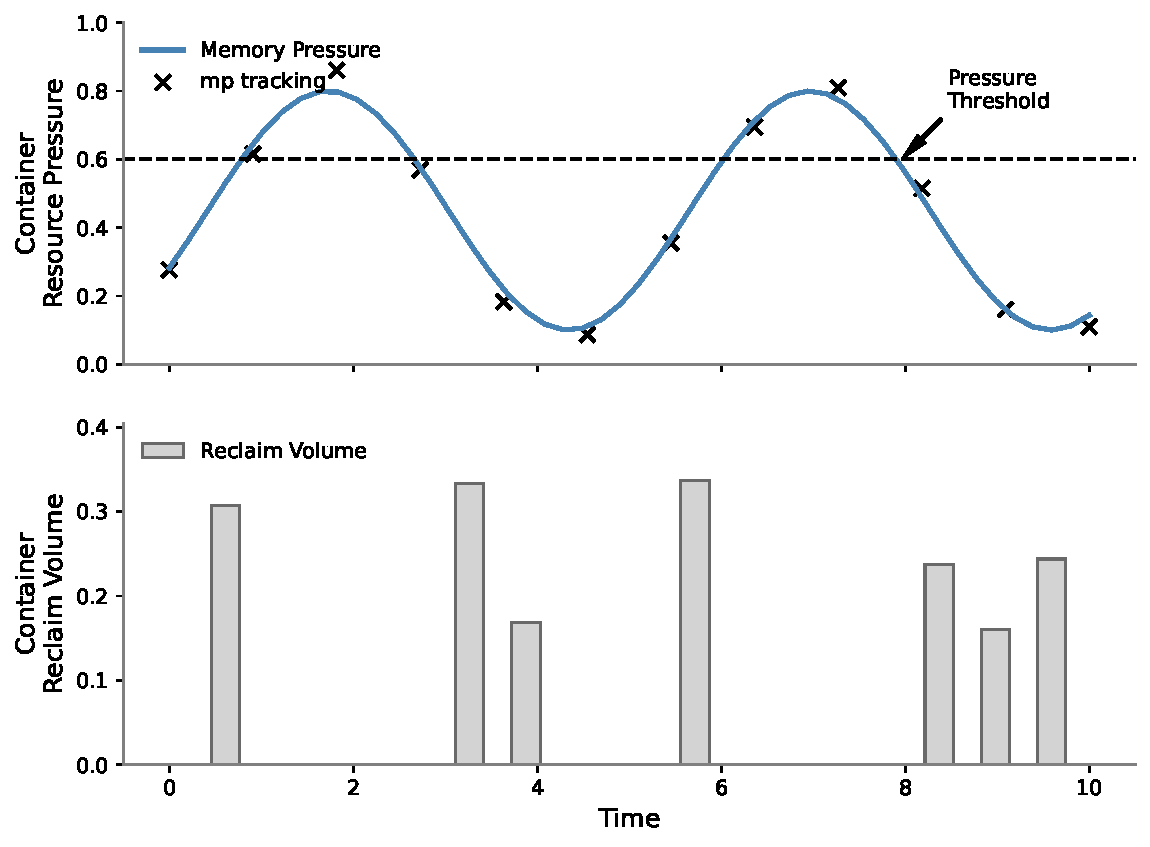
\includegraphics[width=0.95\textwidth]{压力与回收.pdf}
\caption{内存压力与页面回收调控机制}
\label{fig:pressure_work_set}
\end{figure}

图\ref{fig:pressure_work_set}展示了本模型的核心设计目标及运行机制。通过建立一个压力感知的闭环调控系统,该模型能够根据测量的内存压力值动态调整内存使用边界。当系统内存压力超过预设阈值时,模型逐步放宽内存限制以应对增长的工作集需求;反之,当内存压力低于目标值时,模型主动收紧内存限制并触发冷页面卸载,从而释放未充分利用的内存资源。这种基于压力的负反馈机制确保了系统能够在不同负载条件下维持接近最优的内存分配状态。

算法\ref{alg:control}详细描述了基于压力量化的动态调控机制。与传统的静态内存分配策略不同,该算法通过实时内存压力指标构建了资源分配的动态反馈系统。算法以固定的时间间隔(默认为6秒)执行一次评估,通过计算当前内存压力与目标压力阈值之间的偏差来确定调整策略和幅度。

\begin{table}[H]
\centering
\caption{调控参数体系}
\label{tab:params}
\begin{tabular}{cccc}
\toprule
参数 & 符号 & 默认值 & 作用域 \\
\midrule
目标压力 & \(mem\_pressure\_target\) & 0.1\% & 全局 \\
最大收缩率 & \(M_p\) & 0.01 & 缩容阶段 \\
最大扩张率 & \(M_b\) & 1.0 & 扩容阶段 \\
收缩灵敏度 & \(C_p\) & 10 & 缩容触发 \\
扩张灵敏度 & \(C_b\) & 20 & 扩容触发 \\
\bottomrule
\end{tabular}
\end{table}

表\ref{tab:params}列出了算法的关键参数体系。目标压力值(\(mem\_pressure\_target\))作为全局调控基准,默认设置为0.1\%,表示系统期望维持的同步回收延迟占比。灵敏度系数(\(C_p\)和\(C_b\))控制系统对压力变化的响应程度:扩张灵敏度\(C_b = 20\)表示当实际压力达到目标值20倍时,触发最大扩容比例;收缩灵敏度\(C_p = 10\)表示当压力降至目标值1/10时,系统执行最大缩容操作。最大调整率参数(\(M_b\)和\(M_p\))限定了单次调整的幅度上限:最大扩张比例\(M_b = 1.0\)允许在单次调整中将内存限制扩大至原值的两倍,以快速响应突发性工作负载;最大收缩比例\(M_p = 0.01\)将单次缩容限制在1\%以内,确保系统稳定性并避免服务质量剧烈波动。

\begin{algorithm}[H]
    \caption{基于压力的内存调控算法}
    \label{alg:control}
    \Input{\(mem\_pressure\), \(mem\_pressure\_target\), \(C_b\), \(C_p\), \(M_b\), \(M_p\), \(min\_size\), \(max\_size\)}
    \Output{Memory Limit \(Limit\)}
    \While{\textrm{true}}{
        \(mem\_pressure\) get from proc file system;\\
        \If{\(mem\_pressure > mem\_pressure\_target\)}{
            \(\eta \leftarrow \min\left(\left(\frac{mem\_pressure/mem\_pressure\_target}{C_b}\right)^2, 1\right)\)*\(M_b\)\;
            \(Limit \leftarrow \min(max\_size, Limit \times (1 + \eta))\)\;
            }
        \Else{
            \(\eta \leftarrow \min\left(\left(\frac{mem\_pressure\_target/mem\_pressure}{C_p}\right)^2, 1\right)\)*\(M_p\)\;
            \(Limit \leftarrow \max(min\_size, Limit \times (1 - \eta))\)\;
            }
        Apply new memory limit \(Limit\)\;
    }
\end{algorithm}

算法通过二次函数映射将压力偏差转换为调整系数,采用平方关系确保对小偏差具有较低敏感度,而对大偏差则产生更强响应。这种设计避免了因瞬时波动导致的频繁调整,同时保证了对持续性压力变化的及时响应。算法还通过积分机制累积一定时间窗口内的压力变化,以检测持续性负载趋势而非瞬时波动,进一步提高了系统稳定性。

需要强调的是,上述算法设计具有高度可配置性,允许根据不同应用场景和性能需求进行参数调整。在高实时性要求的环境中,可以配置较高的扩张灵敏度和较低的收缩灵敏度,实现对压力增长的快速响应;而在资源受限且对性能波动容忍度较高的场景中,则可采用更积极的收缩策略以最大化资源利用率。通过这种参数化设计,算法能够适应从延迟敏感型在线服务到吞吐量导向的批处理任务等各类工作负载特性。

此调控模型的优势在于将内存管理决策建立在直接测量的系统压力之上,而非依赖难以精确估计的工作集大小。这种方法既避免了传统启发式算法在异构系统上的适应性问题,又实现了对资源利用的精细调控。未来研究方向包括引入机器学习技术实现参数的自适应调整,以及将该模型扩展至更广泛的资源管理领域,如CPU、I/O带宽等多维资源的协同优化。

\section{基于重用距离的自适应页面回收策略}
\label{sec:基于重用距离的冷热页面优化}

\subsection{重用距离}

设计一种通用的、高效的冷热页面识别算法具有挑战性。传统方法通常通过分析负载的特征来提出启发式的识别算法。Linux早期提出了基于重用距离(Reuse Distance)\citing{jiang2002lirs,jiang2005clockpro}的冷热页面识别算法,但由于其实现复杂度和所需额外辅助信息较多,难以在实际系统中直接应用。本研究将重用距离的概念引入页面替换策略的设计中,旨在实现文件页面与匿名页面回收之间的自适应平衡。重用距离能够有效刻画页面访问模式及其在页面替换中的优先级。

对于一段内存访问序列:
\[
  A \;=\;\{\,a_1,\,a_2,\,\dots,\,a_n\},
\]
其中 \(a_i\) 表示第 \(i\) 次访问的页面。令 \(P\) 为目标页面,其重用距离可以形式化地定义为:
\begin{align}
\label{eq:rd_def}
  RD(P) 
  &= 
  \min_{j>i}\Bigl\{\,j - i
    \;\Bigm|\;
    a_i = P,\;
    a_j = P,\;
    i < j
  \Bigr\}.
\end{align}

页面的重用距离与其访问频率密切相关。直观而言,若\(RD(P)\)较短,则表明页面\(P\)在近期被频繁访问,具有较高的局部性;若\(RD(P)\)较长,则表明其访问稀疏,通常可作为回收候选。

\begin{figure}[htbp]
  \centering
  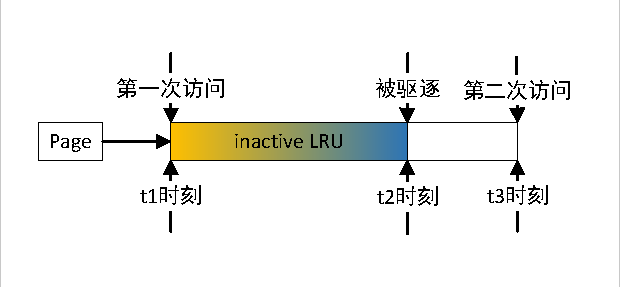
\includegraphics[width=0.5\textwidth]{重用距离.pdf}
  \caption{重用距离示意图}
  \label{fig:refault_distance}
\end{figure}

如图\ref{fig:refault_distance}所示,页面的重用距离可以直观地理解为\(t_1\)到\(t_3\)时间段内,访问过的不同页面的数量。通过分析页面重用距离的分布,可以识别出访问模式的改变,从而及时调整页面替换策略。然而,在大型系统中精确计算每个页面的重用距离会引入显著的空间开销和计算开销。为此,本研究提出了一种基于页面在活动链表和非活动链表间迁移行为的近似策略,通过观察页面在链表中的位置变化来间接推断其访问频度。当页面在非活动链表上被替换(即被驱逐)时,如果它在短期内再次被访问(即发生缺页异常),则说明在两次访问之间,系统至少经历了与非活动链表长度相当数量的页面访问。因此,可以通过统计缺页异常的次数和间隔来近似估计页面的访问频率。

\subsection{重用距离的近似推导}

为了简化分析,首先假设非活动链表长度固定,并且暂不考虑活动链表向非活动链表的页面降级。这种简化有助于更直观地分析非活动链表上的页面替换与访问行为。图\ref{fig:现象1}与图\ref{fig:现象2}展示了两种核心场景。

\begin{figure}[htbp]
  \centering
  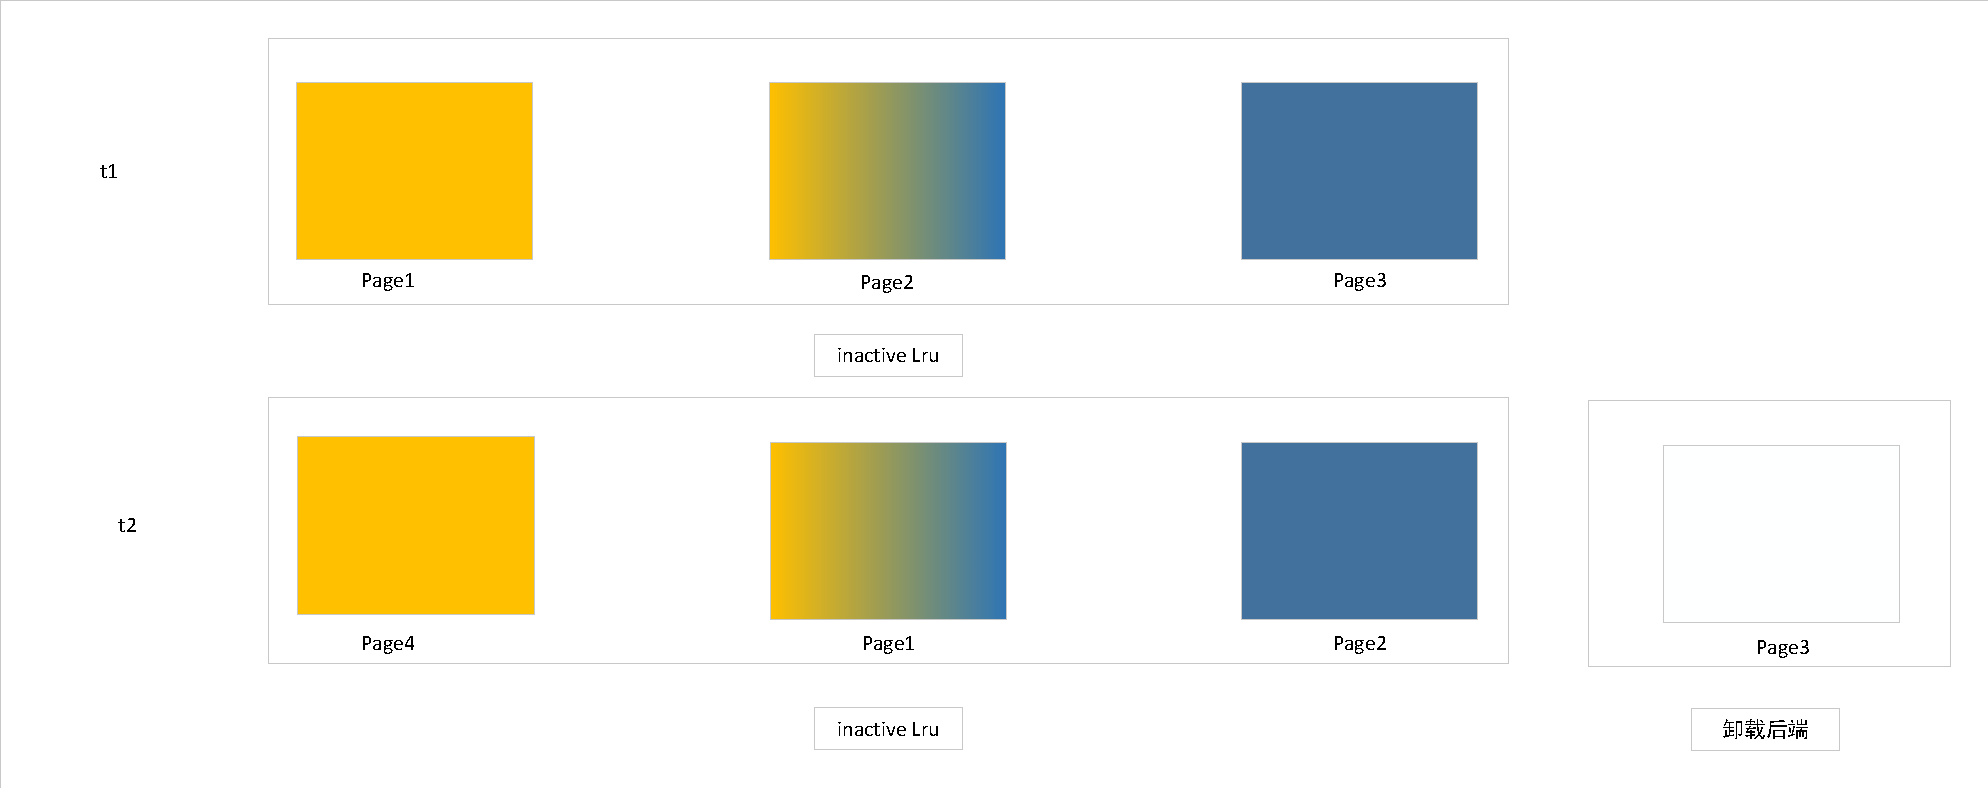
\includegraphics[width=0.5\textwidth]{现象1.pdf}
  \caption{场景一:页面首次插入非活动链表}
  \label{fig:现象1}
\end{figure}

\begin{figure}[htbp]
  \centering
  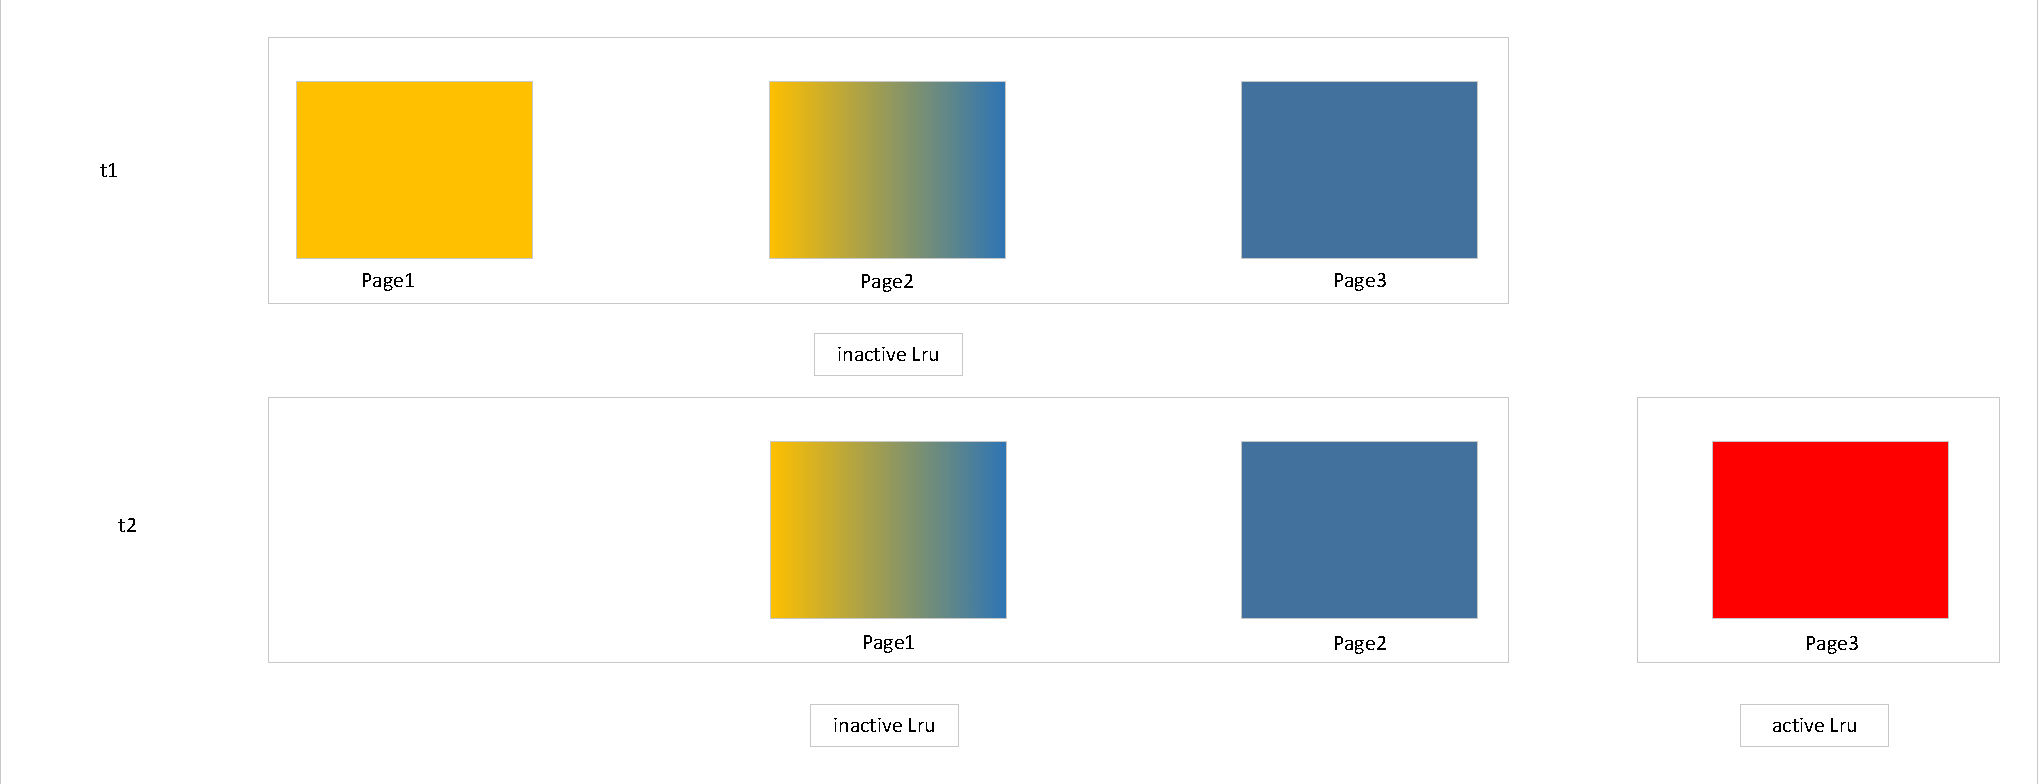
\includegraphics[width=0.5\textwidth]{现象2.pdf}
  \caption{场景二:页面在非活动链表上再次被访问并提升到活动链表}
  \label{fig:现象2}
\end{figure}

\textbf{场景一}(图\ref{fig:现象1})描述了页面首次被访问并插入到非活动链表头部。由于链表长度固定,原链表中的页面整体向尾部移动,最末尾的页面被驱逐出内存。

\textbf{场景二}(图\ref{fig:现象2})描述了页面在非活动链表上再次被访问后,被提升到活动链表,链表长度相应缩短。与此同时,所有比被提升页面更晚进入非活动链表的页面均向尾部移动,更接近被驱逐的状态。

在时间区间\([t_1, t_2]\)内,非活动链表上的页面只可能有两种状态:被驱逐(表明至少加载了一个新的页面)或被提升至活动链表(表明被再次访问)。令\(E(t_1,t_2)\)表示该区间内的驱逐次数,\(A(t_1,t_2)\)表示该区间的页面提升次数。由于每次驱逐对应至少一次新页面的载入,每次提升对应至少一次对非活动链表中页面的访问,因此可以合理地认为,在\([t_1,t_2]\)时间段内发生的页面访问总数\(V(t_1, t_2)\)满足以下不等式:
\[
V(t_1, t_2) \ge E(t_1,t_2) + A(t_1,t_2)
\]

这个不等式给出了页面访问次数的下界估计。

在真实系统中,还需要考虑一直停留在活动链表、从未降级的页面访问量。然而,对于访问极频繁的页面,由于它们并不会进入非活动链表,无需担心其再次访问情形的遗漏,因此对这部分页面的统计影响相对有限。

当页面\(p\)被驱逐时,记录其驱逐时刻\(t_1\)对应的全局计数器\(\mathrm{count}(t_1)\),该计数器累积了系统自启动以来的总驱逐次数和提升次数。

若该页面于时刻\(t_2\)再次被访问,则同样记录\(\mathrm{count}(t_2)\)。此时,基于上述计数器,定义页面\(p\)的重用距离(Refault Distance)为:
\begin{align}
  \label{eq:refault_distance}
  RD_{\mathrm{refault}}(p)
  &= 
  \mathrm{count}(t_2)
  \;-\;
  \mathrm{count}(t_1).
\end{align}

该距离衡量了页面从被驱逐到再次访问期间,系统所经历的页面访问次数的下界。

由于页面在非活动链表中从头部移动到尾部直至被驱逐的过程,可以近似看作是经历了一系列其他页面的访问,因此,非活动链表的长度\(L_{\mathrm{inactive}}\)可以作为页面在缓存中停留期间所经历的页面访问次数的估计。综合考虑页面在非活动链表中的移动和缺页异常期间的访问,可以得到页面\(p\)的总访问距离的近似形式:
\begin{align}
  \label{eq:dtotal}
  RD_{\mathrm{total}}(p)
  &= 
  L_{\mathrm{inactive}}
  \;+\;
  \bigl(\mathrm{count}(t_2) \;-\; \mathrm{count}(t_1)\bigr).
\end{align}

当非活动链表长度较小时,\(\mathrm{count}(t_2) - \mathrm{count}(t_1)\)的增量会相对较大,这表明页面需要具有更高的访问频率才能在非活动链表中停留足够长的时间而不被快速驱逐。

\subsection{替换决策与回收策略}

为了确定页面是否应该继续保留在内存中,需要综合考虑其在非活动链表中的重用距离和活动链表的长度。如果页面希望继续留在内存中,其总访问距离不应超过活动链表和非活动链表的总长度:
\begin{align}
  \label{eq:active_condition_1}
  L_{\mathrm{inactive}}
  \;+\;
  \bigl(\mathrm{count}(t_2) \;-\; \mathrm{count}(t_1)\bigr)
  &\;\;\le\;\;
  L_{\mathrm{inactive}}
  \;+\;
  L_{\mathrm{active}}
\end{align}

化简后可得:
\begin{align}
  \label{eq:active_condition}
  \mathrm{count}(t_2) - \mathrm{count}(t_1)
  \;\le\;
  L_{\mathrm{active}}
\end{align}

这意味着,只有当页面的重用距离小于等于活动链表长度时,才认为其访问频率足够高,值得继续保留在内存中。

在Linux内核中,可以将该方法与\(\mathrm{swappiness}\)等内核参数结合,动态调整文件页与匿名页的回收策略。例如:
\begin{equation}
  \label{swappiness1}
  \mathrm{swappiness} = \min \left( \mathrm{swappiness} \times (1 + \mathrm{refault\_active}), \; 150 \right)
\end{equation}

其中,\(\mathrm{refault\_active}\)表示在最近一段时间内页面发生缺页异常的比例,通过该值可以对回收过程进行动态调节。当系统检测到高缺页异常率时,表明当前回收策略过于激进,可能错误地驱逐了热页面,此时应适当增加\(\mathrm{swappiness}\)值以提高文件页的保留优先级;反之,当缺页异常率较低时,可以适当减小\(\mathrm{swappiness}\)值以加速匿名页的回收。

综上所述,本研究提出的基于重用距离近似估计的页面替换策略,能够在较低开销下有效识别冷热页面,并指导文件页和匿名页的回收决策,从而提高内存利用率和系统整体性能。

\subsection{基于阴影条目的重用距离追踪内核实现}

前文提出的基于重用距离的冷热页面识别与自适应回收算法,需要在内核中实现多个关键机制以支持其运行。本节将详细介绍全局计数维护、页面驱逐与再加载的处理流程,以及阴影条目的复用机制。

\subsubsection{全局计数维护}

为了实现基于重用距离的页面替换策略,需要在内核中维护以下关键计数信息:

\begin{enumerate}
  \item 全局的驱逐和提升次数之和(记为\(\mathrm{nr\_count}\))。
  \item 上次缺页异常统计的次数之和(记为\(\mathrm{nr\_refault\_last}\))。
  \item 当前时刻累积的缺页异常次数之和(记为\(\mathrm{nr\_refault}\))。
  \item 文件页面被驱逐时对应的驱逐与提升次数之和。
\end{enumerate}

其中,前三项计数直接存储在\texttt{lruvec}结构体的原子变量中。每当页面发生驱逐或提升事件时,为了保证并发访问时的计数准确性,需要对\(\mathrm{nr\_count}\)执行原子递增操作。当页面再次加载时,如果满足公式\ref{eq:active_condition}的条件,则表明该页面在被驱逐后不久即被再次访问,此时系统会将其视为一次缺页异常,并相应地增加\(\mathrm{nr\_refault}\)计数。通过计算\(\mathrm{nr\_refault}\)和\(\mathrm{nr\_refault\_last}\)的差值,可以动态评估文件页的\(refault\_active\),进而通过公式\ref{swappiness1}调整文件页和匿名页的回收比例。

\subsubsection{阴影条目管理}

Linux内核中的page cache使用前缀树(Radix Tree)作为索引结构,通过文件偏移量来查找对应的\texttt{struct page}指针。图\ref{fig:前缀树}展示了通过前缀树查找文件偏移量为2222的页面在page cache中的对应项,每级节点根据页偏移量的特定位段进行寻址。前缀树通过路径压缩等优化技术,能够在节点分布稀疏的情况下有效降低内存占用。形式化地,第\(i\)级节点的选择可表示为:
\[
\text{node}_i = \text{node}_{i-1}.\text{slots}[(p_{\text{off}} \gg \text{shift}_i) \& \text{MASK}]
\]

其中,\(\text{node}_i\)表示第\(i\)级节点,\(\text{node}_{i-1}\)表示其父节点,\(\text{slots}\)表示节点中的槽位数组,\(p_{\text{off}}\)表示页偏移量,\(\text{shift}_i\)表示第\(i\)级节点的位移量,\(\text{MASK}\)是一个位掩码常量,用于提取页偏移量中的相关位段。

\begin{figure}[htbp]
  \centering
  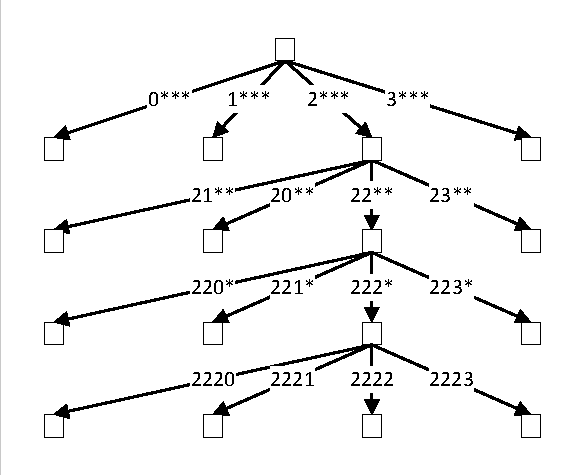
\includegraphics[width=\textwidth]{前缀树.pdf}
  \caption{page cache 的前缀树结构示意}
  \label{fig:前缀树}
\end{figure}

最终得到的值是\texttt{struct page}的指针。为了节省内存空间,\texttt{struct page}数据结构采用了紧凑的内存布局,并实现了16字节对齐,因此指针的最后4位全为0。内核利用\texttt{struct page}指针的低两位作为标志位。表\ref{tab:标志位}详细说明了这些标志位的含义与用途。为了实现页面被驱逐时记录全局计数的需求,本研究复用了前缀树指针槽的标志位。

\begin{table}[htbp]
  \centering
  \caption{struct page指针低两位标志位含义}
  \label{tab:标志位}
  \begin{tabular}{cc}
    \toprule
    \textbf{标志位} & \textbf{说明} \\
    \midrule
    \texttt{00} & 指向 \texttt{struct page} 的正常指针 \\
    \texttt{01} & 内部节点 \\
    \texttt{10} & 阴影条目(shadow entry) \\
    \texttt{11} & 保留 \\
    \bottomrule
  \end{tabular}
\end{table}

在\_\_remove\_mapping函数中,当文件页面即将被从page cache中移除时,系统执行以下步骤:

\begin{enumerate}
  \item 读取当前全局计数器\(\mathrm{nr\_count}\)的值,并将其左移两位,为标志位预留空间。
  \item 将移位后的计数器值与\texttt{10}进行按位或运算,生成阴影条目,并将其写回前缀树的对应槽位。
  \item 对全局计数器\(\mathrm{nr\_count}\)进行原子递增操作,表示发生了一次页面驱逐。
  \item 将页面从活动链表或非活动链表中移除,完成驱逐过程。
\end{enumerate}

\begin{figure}[htbp]
  \centering
  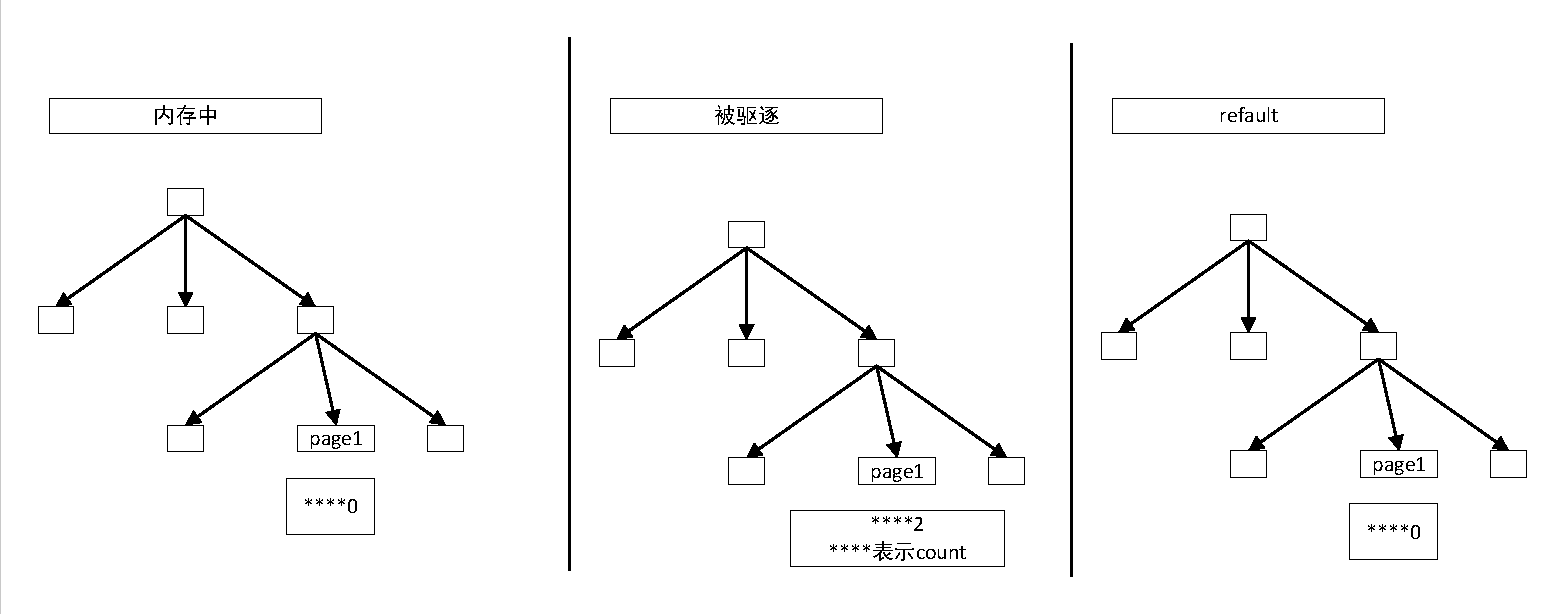
\includegraphics[width=\textwidth]{复用.pdf}
  \caption{利用阴影条目存储驱逐时的 \(\mathrm{nr\_count}\)}
  \label{fig:复用}
\end{figure}
当后续对同一文件偏移发生缺页异常而需要载入页面时,系统执行以下步骤:

\begin{enumerate}
  \item 内核检测到前缀树对应槽位存储的指针标志位不是\texttt{00},判断其为阴影条目。
  \item 提取阴影条目中的数值,并将其右移两位,得到页面被驱逐时的全局计数器值\(\mathrm{count}(t_1)\)。
  \item 计算当前全局计数器值\(\mathrm{count}(t_2)\)与\(\mathrm{count}(t_1)\)的差值,如果该差值不超过活动链表长度\(L_{\mathrm{active}}\),则认为该页面在短期内被再次访问,将其提升至活动链表,并对\(\mathrm{nr\_refault}\)计数器进行原子递增操作。
  \item 如果差值超过\(L_{\mathrm{active}}\),则仅将该页面添加到非活动链表,不更新\(\mathrm{nr\_refault}\)计数器。
\end{enumerate}

如图\ref{fig:复用}所示,页面在内存中时使用普通指针(标志位\texttt{00});被驱逐后,其在前缀树中的对应项被替换为阴影条目(标志位\texttt{10});当页面被重新加载时,内核可以根据阴影条目中记录的信息计算重用距离,并进行相应的处理。该方法通过复用前缀树指针的低位标志位,避免了在\texttt{struct page}结构中引入额外的字段来存储驱逐计数,从而最大程度地减少了内存开销。


\subsubsection{Shrinker回收机制}

在上一节中,介绍了如何通过复用前缀树指针的低位标志位来存储页面驱逐时的全局计数器值。然而,这种方法会导致前缀树中的阴影条目数量不断累积。如果不及时清理这些阴影条目,可能会导致前缀树过度膨胀,占用过多的内存资源。
\begin{table}[htbp]
  \centering
  \caption{struct shrink\_control 结构体主要字段说明}
  \label{tab:shrink_control_struct}
  \begin{tabular}{ccc}
    \toprule
    \textbf{成员} & \textbf{类型} & \textbf{说明} \\
    \midrule
    gfp\_mask & gfp\_t & 本次内存分配的掩码,指示约束条件 \\
    nid & int & 所在的 NUMA 节点 \\
    nr\_to\_scan & unsigned long & 期望本轮扫描并回收的对象数 \\
    nr\_scanned & unsigned long & 实际扫描对象数量 \\
    memcg & struct mem\_cgroup * & 针对特定 memcg 的回收(若有) \\
    \bottomrule
  \end{tabular}
\end{table}

为了解决阴影条目累积导致的内存浪费问题,本研究利用Linux内核提供的Shrinker机制来实现对阴影条目的自动回收。Shrinker是Linux内核内存回收子系统中的统一回调接口,用于管理内核缓存对象(如inode、dentry等)的回收。
\begin{table}[htbp]
  \centering
  \caption{struct shrinker 结构体主要字段说明}
  \label{tab:shrinker_struct}
  \begin{tabular}{ccc}
    \toprule
    \textbf{成员} & \textbf{类型} & \textbf{说明} \\
    \midrule
    count\_objects & 函数指针 & 返回可回收对象数,若无可回收则返回 SHRINK\_EMPTY \\
    scan\_objects & 函数指针 & 实际扫描并回收对象,返回已释放数量 \\
    batch & long & 每次回收的批次大小,默认为 0(使用默认值) \\
    seeks & int & 反映对象重建开销,影响回收优先级 \\
    flags & unsigned & Shrinker 能力标志(NUMA 感知等) \\
    list & struct list\_head & 内核内部使用,用于将 shrinker 链接到全局列表 \\
    id & int & 在 memcg 上下文中的 shrinker 标识 \\
    nr\_deferred & atomic\_long\_t * & 延迟对象数计数 \\
    \bottomrule
  \end{tabular}
\end{table}
Shrinker机制通过struct shrink\_control(表\ref{tab:shrink_control_struct})与struct shrinker(表\ref{tab:shrinker_struct})两个核心数据结构向回收框架注册接口,内核则在内存压力情形下调用对应的回调函数执行清理动作。

\begin{figure}[htbp]
  \centering
  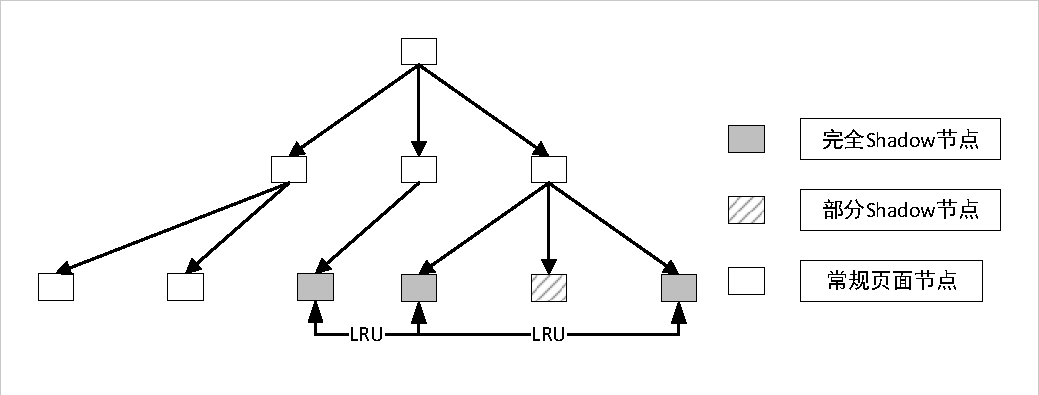
\includegraphics[width=\textwidth]{Shrinker设计.pdf}
  \caption{Shrinker机制工作原理示意图}
  \label{fig:shrink}
\end{figure}

本研究实现的\texttt{scan\_objects}函数利用了Linux内核现有的LRU链表机制实现高效回收。如图\ref{fig:shrink}所示,它不直接遍历整个前缀树,而是只操作已被添加到专用LRU链表的仅包含阴影条目的前缀树节点。为了避免回收操作对正常页面访问造成影响,只有当一个前缀树节点完全由阴影条目组成时,才会被添加到专用的LRU链表中进行回收。由于LRU链表提供了按访问顺序排列的节点列表,因此可以在\(O(1)\)时间内找到最近最少使用的纯阴影节点。

\texttt{count\_objects}函数负责估算可回收的阴影条目数量。它根据系统当前的内存压力水平,动态计算合理的阴影节点数量上限,并只回收超出这一上限的节点。

\section{本章小结}
\label{sec:本章小结}

本章详细介绍了基于内存压力的自适应主动冷页面卸载框架的设计与实现。首先,介绍了利用proc文件系统实现的mpfs模块,提供了用户态与内核态之间的标准交互接口。mpfs模块允许用户态程序实时获取内存压力信息,并动态调整采样周期和压力阈值,为用户态的调控策略提供了基础。随后,提出了基于内存压力的动态调控模型,利用负反馈机制,根据实时内存压力动态调整内存使用范围,实现了主动的冷页面卸载。该模型通过参数化设计,可以灵活适应不同的应用场景和性能需求。最后,详细介绍了基于重用距离的自适应页面回收策略。通过近似计算页面的重用距离,实现了文件页和匿名页的自适应平衡回收。为了支持该策略,本研究在内核中实现了全局计数维护、阴影条目管理和Shrinker回收机制。通过复用前缀树指针的低位标志位,避免了在\texttt{struct page}结构中引入额外字段,最大程度地减少了内存开销。

本章提出的框架和算法,为实现高效、自适应的内存管理提供了可行的方案。通过将内存压力作为核心调控指标,结合重用距离进行页面回收决策,能够在保证系统性能的同时,显著提高内存资源的利用率。未来的研究方向包括引入机器学习技术实现参数的自适应调整,以及将该模型扩展至更广泛的资源管理领域。
